\documentclass{article}

\usepackage{graphicx,fullpage,natbib,amsmath,siunitx,upquote,lineno}

\title{\texttt{IsoplotR}: a free and open toolbox for geochronology}

\author{Pieter Vermeesch\\Department of Earth Sciences\\
  University College London\\
  Gower Street, London WC1E 6BT\\
  \texttt{p.vermeesch@ucl.ac.uk}
}

\linenumbers

\begin{document}
\maketitle

\begin{abstract}
  This paper reviews the basic principles of radiometric geochronology
  as implemented in a new software package called \texttt{IsoplotR},
  which was designed to be free, flexible and future-proof.
  \texttt{IsoplotR} is free because it is written in non-proprietary
  languages (\texttt{R}, \texttt{Javascript} and \texttt{HTML}) and is
  released under the GPL license. The program is flexible because its
  graphical user interface (GUI) is separated from the command line
  functionality, and because its code is completely open for
  inspection and modification. To increase future-proofness, the
  software is built on free and platform-independent foundations that
  adhere to international standards, have existed for several decades,
  and continue to grow in popularity. \texttt{IsoplotR} currently
  includes functions for U-Pb, Pb-Pb,
  \textsuperscript{40}Ar/\textsuperscript{39}Ar, Rb-Sr, Sm-Nd, Lu-Hf,
  Re-Os, U-Th-He, fission track and U-series disequilibrium dating. It
  implements isochron regression in two and three dimensions,
  visualises multi-aliquot datasets as cumulative age distributions,
  kernel density estimates and radial plots, and calculates weighted
  mean ages using a modified Chauvenet outlier detection criterion
  that accounts for the analytical uncertainties in heteroscedastic
  datasets. Overdispersion of geochronological data with respect to
  these analytical uncertainties can be attributed to either a
  proportional underestimation of the analytical uncertainties, or to
  an additive geological scatter term. \texttt{IsoplotR} keeps track
  of error correlations of the isotopic ratio measurements within
  aliquots of the same samples. It uses a statistical framework that
  will allow it to handle error correlations between aliquots in the
  future. Other ongoing developments include the implementation of
  alternative user interfaces and the integration of \texttt{IsoplotR}
  with other data reduction software.
\end{abstract}

\section{Introduction}

Geology is, in essence, a historical science in which timing is of the
utmost importance.  Geochronology underpins the study of Earth history
and puts fundamental constraints on the rate of biological evolution
\citep{chen2012,gradstein2012}. Technological advances in mass
spectrometry, such as the widespread availability of multi-collector
instruments, are ever increasing the precision of the isotopic data
that form the basis of the chronostratigraphic timescale. A plethora
of mathematical-statistical techniques are available to extract
chronological constraints from these isotopic measurements. Examples
of this include isochrons, concordia diagrams, age spectra and density
estimates. Implementing these methods in a rigorous and
self-consistent manner requires appropriate software. For many years,
a \texttt{Microsoft Excel} add-in called \texttt{Isoplot} has served
this purpose extremely well.\\

Developed by Kenneth R. Ludwig over a period of two decades,
\texttt{Isoplot} is a user-friendly toolbox that allows geologists to
calculate and visualise geochronological data within a familiar
spreadsheet environment \citep{ludwig1988, ludwig1999, ludwig2003,
  ludwig2012}.  Few computer programs have been as widely used in the
Earth Sciences as \texttt{Isoplot}. Written in Visual Basic for
Applications (\texttt{VBA}), \texttt{Isoplot} takes isotopic data as
input and produces publication-ready figures as output. Unfortunately,
recent versions of \texttt{Excel} are incompatible with
\texttt{Isoplot}, whose creator has retired and no longer maintains
the code. These software issues are a major problem for the field of
radiometric geochronology, to the point where some laboratories keep
an old \texttt{Windows~XP} computer with \texttt{Excel~2003} around
for the sole purpose of running \texttt{Isoplot}.\\

This paper introduces a new computer code called \texttt{IsoplotR} as
a free, open and more future-proof alternative for \texttt{Isoplot}.
The principal aim of this paper is to provide a general overview of
the design philosophy and basic operating principles behind the
software, rather than a detailed manual of all its components.
Section~\ref{sec:architecture} discusses the software architecture,
which uses a modular design with future-proofness and extendability in
mind. Section~\ref{sec:input} presents three fundamental types of
input format that are used by \texttt{IsoplotR} to capture the
covariance structure of isotopic ratio data. We will see that this
covariance structure plays a fundamental role in all of
\texttt{IsoplotR}'s methods.\\

Section~\ref{sec:regression} reviews the important subject of linear
regression, which underpins the construction of
isochrons. \texttt{IsoplotR} currently implements three different
types of error weighted linear regression algorithms that account for
error correlations between variables and between aliquots in two or
three dimensions.  Section~\ref{sec:overdispersion} explains how these
three methods represent different approaches of dealing with
overdispersion.  Section~\ref{sec:averaging} introduces a weighted
mean plot to visualise multiple age estimates and proposes a heuristic
method to detect outliers.  Section~\ref{sec:confidence} presents
three approaches to construct confidence intervals for isochron ages,
weighted means and so forth.  It introduces a profile log-likelihood
method for the calculation of asymmetric confidence
intervals.\\

Section~\ref{sec:density} discusses three further methods to visualise
multi-aliquot collections of ages. Cumulative age distributions (CADs)
and kernel density estimates (KDEs) show the frequency distribution of
the age measurements but do not explicitly take into account the
analytical uncertainties. The radial plot is introduced as a more
appropriate data visualisation tool for `heteroscedastic' data
(i.e. data with unequal measurements uncertainties). The radial plot
provides a good vehicle to assess the dispersion of multi-aliquot
datasets. Overdispersed datasets require further processing with
continuous or discrete mixture models that are discussed in
Section~\ref{sec:mixtures}.\\

Sections~\ref{sec:PD}-\ref{sec:FT} provide
specific details about the Rb-Sr, Sm-Nd, Lu-Hf, Re-Os,
\textsuperscript{40}Ar/\textsuperscript{39}Ar, U-Pb, Pb-Pb, U-Th-He,
fission track and U-series dating methods. Section~\ref{sec:detritals}
introduces a selection of statistical methods to help interpret
collections of multiple geochronological datasets that are useful in
detrital geochronology. Finally, Section~\ref{sec:future} sets out a
roadmap for future developments to improve the accuracy and precision
of geochronological data, and to provide closer integration of
\texttt{IsoplotR} with earlier steps of the data processing chain.

\section{Software architecture}
\label{sec:architecture}

There are three ways to use \texttt{IsoplotR}: online, offline and
from the command line.\\

The online version can be accessed at
\texttt{http://isoplotr.london-geochron.com} (see Appendix~A), and is
convenient in several ways. First, it requires no software
installation. Second, the \texttt{IsoplotR} website is perfectly
platform-independent. It renders on any modern HTML-5 compatible web
browser, including those installed on smartphones and tablet
computers. Third, by using the online version, the user is guaranteed
to have accessed the most up-to-date version of the software.\\

An offline version of the GUI is provided for use on computers that
are not (permanently) connected to the internet. This is often the
case for machines that are connected to mass spectrometers, as a
safety precaution. The offline version of the GUI works by emulating a
web server within the default browser on the user's
system. Installation instructions are provided on the
\texttt{IsoplotR} website and on \texttt{GitHub}.\\

The third way to access the full functionality of \texttt{IsoplotR} is
through the command line within the \texttt{R} programming environment
(see Appendix~B). The command line offers the greatest flexibility to
automate, modify and extend \texttt{IsoplotR}'s functionality.\\

The code base for the GUI and the core data processing algorithms are
surgically separated. The command-line functionality is grouped in a
lightweight package called \texttt{IsoplotR} that may be installed
from the `Comprehensive R Archive Network' (CRAN) by typing
\verb|install.packages('IsoplotR')| at the command prompt. Once
installed, the package can be loaded into memory by typing
\texttt{library(IsoplotR)}. The \texttt{IsoplotR} package has minimal
dependencies and should work on a basic \texttt{R} installation. In
contrast, the GUI is written in \texttt{HTML} and \texttt{Javascript}
and interacts with \texttt{IsoplotR} via an interface package
\citep{chang2017}. It is provided in a second \texttt{R} package
called \texttt{IsoplotRgui} that is available from \texttt{GitHub}
(see the \texttt{IsoplotR} website for details).  \texttt{IsoplotRgui}
is separate from but depends on \texttt{IsoplotR}.\\

The clean separation between the two programs allows \texttt{IsoplotR}
to remain light and easy to install. This is important for any future
\texttt{R} packages that may wish to incorporate \texttt{IsoplotR}
functions. A second reason for keeping the code base of the GUI and
command line functionality separated is that other user interfaces are
planned, for example within \texttt{Excel}
(Section~\ref{sec:future}). Incorporating all these additional
functions into a single package would add unnecessary bulk and
redundancy. \texttt{IsoplotR} and \texttt{IsoplotRgui} are free and
open software.  The computer code for both programs is made available
under the GPL license, which permits re-use and modification provided
that any derived code is released under the same conditions
\citep{gplv3}.

\section{Input formats}
\label{sec:input}

In an abstract sense, \texttt{IsoplotR} is a set of functions $F$ that
take some isotopic data $A$ as input and generate some numerical
and/or graphical output $B$:

\begin{equation}
  B = F(A)
  \label{eq:BFA}
\end{equation}

For example, $A$ could be some
\textsuperscript{40}Ar/\textsuperscript{36}Ar- and
\textsuperscript{39}Ar/\textsuperscript{36}Ar-measurements and $B$
could be the \textsuperscript{40}Ar/\textsuperscript{39}Ar-age. Or $A$
could be some \textsuperscript{87}Sr/\textsuperscript{86}Sr- and
\textsuperscript{87}Rb/\textsuperscript{86}Sr-measurements and $B$ a
vector with the slope and intercept of an isochron fit to these data.
$A$ may also include decay constants, stable isotope ratios and other
parameters that are associated with analytical uncertainty.\\


Regardless of the application, the error propagation of $B$ is as
important as estimation of $B$ itself \citep{ludwig2003}. Without
analytical uncertainties, it is impossible to ascertain whether the
difference between two geochronological dates is real, or simply an
artifact of analytical imprecision. \texttt{IsoplotR} propagates the
analytical uncertainty of $B$ using one of two methods. If $F$ is a
likelihood function, then the error propagation is done by inverting
the (negative) matrix of its second derivatives.  In all other cases,
the error propagation uses a first order Taylor approximation:

\begin{equation}
  \Sigma_B = J_F \Sigma_A J_F^T
  \label{eq:errorprop}
\end{equation}

\noindent where $\Sigma_A$ is the covariance matrix of the input data
$A$, $\Sigma_B$ is the covariance matrix of the estimated parameters
$B$, $J_F$ is the Jacobian matrix with the partial derivatives of the
function $F$ with respect to the measurements $A$, and $J_F^T$ is the
transpose of the Jacobian matrix. If $A$ is a vector of $n$
measurements and $B$ is a vector of $m$ estimated parameters, then
$\Sigma_A$ and $\Sigma_B$ are $n \times n$ and $m \times m$ matrices
with the variances of the $A$s and $B$s on the diagonal and their
covariances on the off-diagonal terms; and $J_F$ is an $n \times m$
matrix of partial derivatives.\\

In order to use Equations~\ref{eq:BFA} and \ref{eq:errorprop},
\texttt{IsoplotR} requires not only the isotopic measurements and
their analytical uncertainties, but also the covariances between these
quantities. For example, in the case of the aformentioned
\textsuperscript{40}Ar/\textsuperscript{39}Ar example, we require the
isotopic ratio measurements ${}^{40}Ar/{}^{36}Ar$ and
${}^{39}Ar/{}^{36}Ar$, their standard errors $s[{}^{40}Ar/{}^{36}Ar]$
and $s[{}^{39}Ar/{}^{36}Ar]$, and their covariance
$cov[{}^{40}Ar/{}^{36}Ar,{}^{39}Ar/{}^{36}Ar]$. Similarly, for the
Rb-Sr example, we require ${}^{87}Rb/{}^{86}Sr$,
$s[{}^{87}Rb/{}^{86}Sr]$, ${}^{87}Sr/{}^{86}Sr$,
$s[{}^{87}Sr/{}^{86}Sr]$ and
$cov[{}^{87}Rb/{}^{86}Sr,{}^{87}Sr/{}^{86}Sr]$.\\

It is generally quite straightforward to obtain the isotopic ratio
estimates and their uncertainties using most data acquisition
software. Unfortunately this is not always the case for the covariance
terms. \texttt{IsoplotR} includes three kinds of input format to
overcome this problem. A first class of input formats consists of a
flat table with five or nine columns:

\[
X,~s[X],~Y,~s[Y],~\rho[X,Y]
\]

\noindent or

\[
X,~s[X],~Y,~s[Y],~Z,~s[Z],~\rho[X,Y],~\rho[X,Z],~\rho[Y,Z]
\]

\noindent where $X$, $Y$ and $Z$ are the isotopic (ratio)
measurements, $s[X]$, $s[Y]$ and $s[Z]$ are their analytical
uncertainties (standard errors); and $\rho[X,Y]$, $\rho[X,Z]$ and
$\rho[Y,Z]$ are the error correlations, which are related to the
covariances as follows:\\

\begin{equation*}
  cov[X,Y] = \rho[X,Y] s[X] s[Y]
  %\label{eq:rho2cov}
\end{equation*}

The remaining two classes of input formats specify the covariance
structure of the data without requiring any actual covariances or
correlation coefficients. For synchronously acquired isotopic data,
such as \textsuperscript{40}Ar/\textsuperscript{39}Ar-data measured by
noble gas mass spectrometry or U-Pb data measured by laser ablation
inductively coupled mass spectrometry (LAICPMS), this is achieved
using redundant ratios. For example, in the case of
\textsuperscript{40}Ar/\textsuperscript{39}Ar-data, let $X$, $Y$ and
$Z$ be three ratios of \textsuperscript{36,39,40}Ar:

\[
X \equiv {}^{36}Ar/^{40}Ar
,~Y \equiv {}^{39}Ar/^{40}Ar
,~Z \equiv {}^{36}Ar/^{39}Ar
\]

\noindent and let $s[X]$, $s[Y]$ and $s[Z]$ be their standard errors.
Then first order Taylor expansion yields:

\begin{equation*}
  \left(\frac{s[Z]}{Z}\right)^2 = \left(\frac{s[X/Y]}{X/Y}\right)^2
  \approx \left(\frac{s[X]}{X}\right)^2 + \left(\frac{s[Y]}{Y}\right)^2 -
  2 \frac{cov[X,Y]}{XY}
  %\label{eq:sZZ2}
\end{equation*}

\noindent from which the covariance between $X$ and $Y$ can be
inferred as

\begin{equation*}
  cov[X,Y] \approx \frac{XY}{2}
  \left[
    \left(\frac{s[X]}{X}\right)^2 +
    \left(\frac{s[Y]}{Y}\right)^2 -
    \left(\frac{s[Z]}{Z}\right)^2
    \right]
  %\label{eq:redundantratios}
\end{equation*}

It is important to note that this approach makes the crucial
assumption that all three standard errors ($s[X]$, $s[Y]$ and $s[Z]$)
are based on the same number of data points. If some data has been
rejected from one ratio but not another, then this relation will not
work.\\

Finally, for isotopic data that are analysed asynchronously, such as
Rb-Sr or Sm-Nd measurements involving liquid chromatography, the
covariance can be obtained from the parent and daughter element
concentrations and the daughter isotopic ratio. For example, in the
case of Rb-Sr data, if the following data are given:

\[
X \equiv Rb~[\text{ppm}]
,~Y \equiv Sr~[\text{ppm}]
,~Z \equiv ({}^{87}Sr/{}^{86}Sr),
\]

\noindent then the \textsuperscript{87}Rb/\textsuperscript{86}Sr-ratio
is given by:

\begin{equation}
  W \equiv \left({}^{87}Rb/{}^{86}Sr\right) = 
  \frac{X}{Y} \frac{M(Rb)}{M(Sr)}
  \frac{
    1+Z\left[1+({}^{84}Sr/{}^{87}Sr)+({}^{88}Sr/{}^{87}Sr) \right]
  }{
    1+({}^{85}Rb/{}^{87}Rb)
  }
  \label{eq:ID}
\end{equation}

\noindent where $({}^{84}Sr/{}^{87}Sr)$, $({}^{88}Sr/{}^{87}Sr)$ and
$({}^{85}Rb/{}^{87}Rb)$ are constant, non-radiogenic isotope ratios,
and $M(Rb)$ and $M(Sr)$ are the molar masses of Rb and Sr,
respectively. Because $Z$ appears in Equation~\ref{eq:ID}, the
covariance ($cov[W,Z]$) between $({}^{87}Rb/{}^{86}Sr)$ and
$({}^{87}Sr/{}^{86}Sr)$ is nonzero and can be estimated using
Equation~\ref{eq:errorprop}.

\section{Regression}
\label{sec:regression}

Isochrons are an important instrument of high precision, high accuracy
geochronology.  Given several aliquots from a single sample, they
allow the non-radiogenic component of the daughter nuclide to be
quantified and separated from the radiogenic component. In its
simplest form, an isochron is obtained by setting out the amount of
radiogenic daughter against the amount of radioactive parent, both
normalised to a non-radiogenic isotope of the daughter element, and
fitting a straight line through these points by least squares
regression \citep{nicolaysen1961}. The slope and intercept then yield
the radiogenic daughter-parent ratio and the non-radiogenic daughter
composition, respectively.\\

There are several ways to fit an isochron.  The easiest of these is
ordinary least squares regression, which weights all data points
equally. In the presence of quantifiable analytical uncertainty, it is
equally straightforward to use the inverse of the y-errors as weights.
It is significantly more difficult to take into account uncertainties
in both the x- and y-variable. The \citet{york1966} method assumes
that the analytical uncertainties of the x- and y-variables are
independent of each other. \texttt{IsoplotR} uses this method to
construct U-Th-He isochrons (Section~\ref{sec:UThHe}).  But for other
chronometers, the assumption of uncorrelated uncertainties is
generally not valid.\\

\citet{york1969} addresses this issue with a bivariate error weighted
linear least squares algorithm that accounts for covariant errors in
both variables (Figure~\ref{fig:1}.a). This algorithm was further
improved by \citet{york2004} to ensure consistency with the maximum
likelihood approach of \citet{titterington1979}. \texttt{IsoplotR}
uses the \citet{york2004} algorithm for its
\textsuperscript{40}Ar/\textsuperscript{39}Ar, Pb-Pb, Rb-Sr, Sm-Nd,
Re-Os and Lu-Hf isochrons (Section~\ref{sec:PD}). The maximum
likelihood algorithm of \citet{titterington1979} was generalised from
two to three dimensions by \citet{ludwig1994} for U-series
disequilibrium dating.  Also this algorithm is implemented in
\texttt{IsoplotR} (Section~\ref{sec:ThU}).\\

Finally, the 3-dimensional maximum likelihood approach of
\citet{ludwig1994} was further modified by \citet{ludwig1998} to fit
so-called `Total Pb-U isochrons', which are constrained to a
radiogenic endmember composition that falls on the concordia line
(Section~\ref{sec:UPb}). In its most sophisticated form, this
algorithm does not only allow for correlated errors between variables,
but also between aliquots. \texttt{IsoplotR} currently uses this
algorithm to propagate decay constant uncertainties in the total Pb-U
isochron ages. Future versions of the program will generalise this
approach to other chronometers as well (Section~\ref{sec:future}).\\

The extent to which the observed scatter in the data can be explained
by the analytical uncertainties can be assessed using a chi-square
test.  To this end, we define the chi-square statistic as:

\begin{equation}
  \chi_{stat}^2 = \left[X - \hat{X}\right] \Sigma_{X}^{-1} \left[X - \hat{X}\right]^T
  \label{eq:Chi2}
\end{equation}

\noindent where $X$ are the data, $\hat{X}$ are the fitted values, and
$\Sigma_X$ is the covariance matrix of $X$. For example, in the case
of a 3-dimensional U-series isochron comprised of $n$ aliquots, $X$ is
a [$1 \times 3n$]-matrix obtained by concatenating all the
\textsuperscript{232}Th/\textsuperscript{238}U-,
\textsuperscript{234}U/\textsuperscript{238}U- and
\textsuperscript{230}Th/\textsuperscript{238}U-ratio measurements, and
$\Sigma_X$ is the corresponding [$3n \times 3n$] covariance matrix.\\

The p-value is defined as the probability of observing a value greater
than $\chi_{stat}^2$ under a chi-square distribution with $df =
k(n-1)$ degrees of freedom, where $k$ is the dimensionality of the
linear fit.  If the p-value falls below a cutoff value of 0.05, say,
then this indicates that the data are `overdispersed' with respect to
the formal analytical uncertainties around the best-fit line. In
contrast, p-values that are much greater than 0.95 are indicative of
`underdispersed' data, possibly reflecting overestimated analytical
uncertainties.\\

An alternative way to assess the degree of over- or underdispersion is
by dividing the chi-square statistic $\chi^2_{stat}$ by the number of
degrees of freedom $df$. The resulting numerical value is called the
`Mean Square of the Weighted Deviates' \citep[MSWD,][]{mcintyre1966}
by geochronologists, but is known as the `reduced chi-square
statistic' elsewhere. MSWD values that are far smaller or greater than
1 indicate under- or overdispersed measurements, respectively.

\section{Dealing with overdispersion}
\label{sec:overdispersion}

Let us consider the simple case of a 2-dimensional dataset
$\{x_1,y_1\},\ldots,\{x_i,y_i\},\ldots,\{x_n,y_n\}$.  Data are
overdispersed with respect to the analytical uncertainties if:

\[
\mathrm{MSWD} \equiv
\sum\limits_{i=1}^n X_i~\Omega_i X_i^T / df > 1
\]

\noindent with

\[
X_i = \left[
  \begin{array}{cc}
    (x_i - \hat{x}_i) &  (y_i - \hat{y}_i)
  \end{array}
  \right],
\]

\noindent where $\hat{x}_i$ and $\hat{y}_i$ are the fitted values, and

\[
\Omega_i \equiv
\left[
  \begin{array}{cc}
    s[x_i]^2 & cov(x_i,y_i) \\
    cov(x_i,y_i) & s[y_i]^2
  \end{array}
\right]^{-1}
\]

\texttt{IsoplotR} provides three alternative strategies (`models') to
deal with overdispersed data. A first way (`model-1') to account for
overdispersion is to inflate all analytical uncertainties by a common
\emph{factor} $f$, which is chosen so as to reduce the MSWD to unity:

\[
\sum\limits_{i=1}^{n} X_i~\Omega_{i,f} X_i^T / df = 1
\]

\noindent with

\[
\Omega_{i,f}
\equiv
\left[
  \begin{array}{cc}
    f^2s[x_i]^2 & f^2cov(x_i,y_i) \\
    f^2cov(x_i,y_i) & f^2s[y_i]^2
  \end{array}
\right]^{-1}
= \Omega_i/f^2
\]

\noindent from which it is easy to show that $f=\sqrt{\mathrm{MSWD}}$.\\


A second option (`model-2') for dealing with overdispersion is to
simply ignore the analytical uncertainties and perform an ordinary
least squares regression. This option is offered for the sake of
completeness but is inherently flawed, because (1) its results may
differ depending on which ratio is chosen as the dependent variable;
(2) it assumes that only the dependent variable is subject to scatter;
which results in (3) unreliable error calculations
\citep[][p. 648]{ludwig2003b}. \\

Finally, a third option (`model-3') is to attribute the overdispersion
to geological scatter in the ages or in the non-radiogenic isotope
composition. The latter hypothesis can be formalised as follows:

\[
\sum\limits_{i=1}^{n} X_i~\Omega_{i,\omega} X_i^T / df = 1
\]

\noindent with

\[
\Omega_{i,\omega} \equiv
\left[
  \begin{array}{cc}
    s[x_i]^2 & cov(x_i,y_i) \\
    cov(x_i,y_i) &  s[y_i]^2 + \omega^2
  \end{array}
\right]^{-1}
\]

\noindent where $\omega$ is the overdispersion \emph{term}, which can
be found iteratively. This term has geological significance and is
reported separately by \texttt{IsoplotR}. The third strategy is
arguably the most sensible one, because geological scatter is a very
common phenomenon.  For example, not all aliquots in a multi-mineral
Rb-Sr isochron may have formed with exactly the same initial
\textsuperscript{87}Sr/\textsuperscript{86}Sr ratio
\citep{mcintyre1966}. As the analytical precision of mass
spectrometers has increased over the years, geochronologists' ability
to detect even the smallest amount of geological dispersion has
steadily grown as well. It is reasonable to assume that this trend
will continue into the future, and that overdispersed datasets will
become ever more common.\\

It is important to note that the overdispersion of geochronological
datasets contains meaningful geological information. For example, the
dispersion of igneous zircon U-Pb dates bears information on the
magmatic residence time of these crystals \citep{matzel2006,
  rioux2012}.  Thus, the increasing prevalence of overdispersed
datasets should be seen as a positive trend rather than a nuisance.

\section{Weighted means}
\label{sec:averaging}

Let $t = \{t_1, ..., t_n\}$ be a set of $n$ age estimates determined
on different aliquots of the same sample, and let $\{s[t_1], ...,
s[t_n]\}$ be their respective analytical
uncertainties. \texttt{IsoplotR} calculates the weighted mean of these
data assuming a Normal distribution with two sources of variance:

\begin{equation}
  p(t_i|\mu,\omega) = \mathcal{N}\left(
  t_i | \mu,\sigma^2=s[t_i]^2+\omega^2 \right)
  \label{eq:weightedmean}
\end{equation}

\noindent where $p(a|b,c)$ stands for ``the probability of observing
$a$ given $b$ and $c$'', $\mu$ is the mean, $\sigma^2$ is the total
variance and $\omega$ is the overdispersion. The latter parameter is
equivalent to its namesake from
Section~\ref{sec:overdispersion}. Equation~\ref{eq:weightedmean} can
be solved for $\mu$ and $\omega$ by the method of maximum likelihood,
yielding two estimates $\hat{\mu}$ and $\hat{\omega}$ and their
approximate covariance matrix. Substituting $X$ for $t$ and $\hat{X}$
for $\hat{\mu}$ in Equation~\ref{eq:Chi2} and dividing by $df = n-2$
degrees of freedom yields the MSWD value for age homogeneity.\\

With regards to error propagation, it is important to make a
distinction between random and systematic sources of uncertainty
\citep{horstwood2016}. Random uncertainties can be reduced to
arbitrarily low levels by averaging an arbitrarily large number of
aliquots. In contrast, systematic uncertainties impose absolute limits
on the precision of geochronological dates.  For example, no absolute
age determination can be more precise than the decay constants
involved. Similarly, for dating methods such as
\textsuperscript{40}Ar/\textsuperscript{39}Ar or fission tracks, no
sample date can be more precise than the $J$ and $\zeta$ calibration
factors, respectively (see Sections~\ref{sec:ArAr} and
\ref{sec:FT}).\\

When solving Equation~\ref{eq:weightedmean}, \texttt{IsoplotR} only
incorporates the random sources of uncertainty into $s[t_i]$.  If the
user wishes to include the systematic uncertainties as well, then this
is done by first computing the isotopic composition corresponding to
the weighted mean age (and its uncertainty), and then re-propagating
the analytical uncertainty of the weighted mean age, this time
including the decay or calibration constant uncertainties.\\

Note that this procedure is unable to handle the systematic
uncertainties associated with stable isotope ratios, molar masses
etc. Those comparably small uncertainties demand a different approach
in which not the ages but the isotopic data are averaged.  Doing so
would require the addition of new input formats that can trace error
correlations between samples (Section~\ref{sec:future}). It would also
require the development of a new generation of low-level
data-processing software \citep{vermeesch2015b,mclean2016}.\\

\texttt{IsoplotR} uses a modified version of Chauvenet's criterion for
outlier detection. The conventional version of this criterion proceeds
as follows:

\begin{enumerate}
\item Compute the (unweighted) arithmetic mean ($\bar{t}$) and
  standard deviation ($s[t]$) of the $n$ age determinations:

  \[
  \bar{t} = \sum_{i=1}^{n} t_i/n \mbox{~and~}
  s[t] = \sqrt{\sum_{i=1}^{n} (t_i-\bar{t})^2/(n-1)}
  \]

\item For each of the $t_i$s, compute the probability $p_i$ that
  $|\tau|>|t_i-\bar{t}|$ for

  \[
  \tau \sim \mathcal{N}(\mu=0,\sigma^2=s[t]^2)
  \]
  
\item Let $p_j \equiv \min(p_1,...,p_n)$. If $p_j<0.05/n$, then reject
  the $j$\textsuperscript{th} date, reduce $n$ by one (i.e., $n
  \rightarrow n-1$) and repeat steps 1 through 3 until all the
  surviving dates pass the third step.

\end{enumerate}

Although this procedure is effective at removing outliers in
\emph{homoscedastic} datasets, in which all datapoints are derived
from a single Normal distribution, it is unable to account for
\emph{heteroscedasticity}, in which different samples are
characterised by different analytical uncertainties ($s[t_i]$ in
Equation~\ref{eq:weightedmean}). \texttt{IsoplotR} introduces a
heuristic modification to Chauvenet's criterion that detects outliers
among heteroscedastic data:

\begin{enumerate}
\item Compute the error-weighted mean of the $n$ age determinations
  $t_i$ using their analytical uncertainties $s[t_i]$ by solving
  Equation~\ref{eq:weightedmean} for $\mu$ and $\omega$ as discussed
  before. Let $\hat{\mu}$ and $\hat{\omega}$ be their respective
  maximum likelihood estimates.
\item For each $t_i$, compute the probability $p_i$ that
  $|\tau|>|t_i-\hat{\mu}|$ for

  \[
  \tau \sim \mathcal{N}(\mu=0,\sigma^2 = s[t_i]^2+\hat{\omega}^2)
  \]
\item Proceed as before.
\end{enumerate}

If the analytical uncertainties are small compared to the scatter
between the dates (i.e., if $\omega \gg s[t_i]$ for all $i$), then
this generalised algorithm reduces to the conventional Chauvenet
criterion. If, on the other hand, the analytical uncertainties are
large and the data do not exhibit any overdispersion, then the
heuristic outlier detection method is similar to \citet{ludwig2003}'s
`modified 2-sigma' approach.\\

The weighted mean calculation is accompanied by a diagram that
consists of a number of rectangular boxes (one for each date) whose
vertical position and height reflect the ages and their analytical
uncertainties, respectively (Figure~\ref{fig:1}.b).  Outliers are
marked in a different colour if so requested. The weighted mean plot
offers an effective way, although arguably not \emph{the} most
effective way, to assess the dispersion of geochronological data. Some
better alternatives are discussed in Section~\ref{sec:density}.

\section{Confidence intervals}
\label{sec:confidence}

By default, \texttt{IsoplotR} requires that the analytical
uncertainties of the input data are provided as standard errors
\citep[\emph{sensu}][p.187]{kenney1954}.  The analytical uncertainties
for the output are reported as paired standard errors and confidence
intervals. In the limit of infinite sample size, the width of a 95\%
confidence interval for the mean, slope and many other statistical
estimates may be obtained by simply multiplying the standard error
with a factor of 1.96.  This forms the rationale for the common
practice in geochronology to quote analytical uncertainty on a `two
sigma' level.  But for smaller sample sizes, this simple method is
usually not accurate.\\

To obtain confidence intervals for model-1 and -2 regression
(Section~\ref{sec:regression}), the propagated uncertainty must be
augmented by the corresponding percentile of a t-distribution with the
appropriate degrees of freedom \citep{ludwig1994}. For model-1
regression of overdispersed datasets, \texttt{IsoplotR} reports the
results as $t \pm x | y | z$ where $t$ stands for the isochron age,
$x$ is the standard error, $y$ is the (95\%) confidence interval
without and $z$ with overdispersion.\\

The studentised confidence intervals do not generally apply to model-3
regression, weighted means and mixture models. In those cases,
\texttt{IsoplotR} uses the profile log-likelihood method
\citep[][p.~200]{galbraith2005}. For example, in the case of the
weighted mean, the log-likelihood corresponding to
Equation~\ref{eq:weightedmean} is given by:

\begin{equation*}
  \mathcal{L} =
    \mbox{const.} - \frac{1}{2}
    \sum\limits_{i=1}^{n}
    \left[
    \ln(s[t_i]^2+\omega^2) +
    \frac{(t_i-\mu)^2}{s[t_i]^2+\omega^2}
    \right]
%  \label{eq:LL}
\end{equation*}

For any value of $\omega$, the profile log-likelihood is given by
maximising $\mathcal{L}$ over all possible values of $\mu$.  Let
$\mathcal{L}_\mbox{max}$ be the overall maximum likelihood estimate.
Then \texttt{IsoplotR} obtains a $100(1-\alpha)\%$ confidence interval
for $\omega$ by collecting all the $\omega$-values whose profile
log-likelihoods exceed $\mathcal{L}_{\mbox{max}} -
\mbox{p}(\chi^2_1,1-\alpha/2)$, where $\mbox{p}(\chi^2_1,1-\alpha/2)$
represents the $100(1-\alpha/2)$-percentile of a chi-square
distribution with one degree of freedom. For example, if $\alpha =
0.05$, then $\mbox{p}(\chi^2_1,0.95) = 3.85$. The resulting confidence
intervals are generally asymmetric.\\

A final point worth mentioning is that \texttt{IsoplotR} enforces a
consistent level of confidence for all numerical and graphical
results. In this spirit, the program plots confidence ellipses at a
95\% (or any other desired) level of confidence, rather than the
`2-sigma' ellipses used elsewhere. The latter only cover 86\% of a
bivariate Normal distribution \citep{horstwood2016}, which may confuse
some users.  Those who insist on using `2-sigma' error ellipses can
easily do so by reducing the desired confidence level from 0.05 to
0.14 in the preferences.

\section{Frequency distributions and radial plots}
\label{sec:density}

Empirical cumulative distribution functions or 'Cumulative Age
Distributions' (CADs) are the most straightforward way to visualise
the frequency distribution of multiple dates. A CAD is a step function
that sets out the rank order of the dates against their numerical
value:

\begin{equation*}
  \mathrm{CAD}(t) = \sum_{i=1}^{n} 1(t<t_i)/n
  %\label{eq:CAD}
\end{equation*}

\noindent where $1(\ast) = 1$ if $\ast$ is true and $1(\ast) = 0$ if
$\ast$ is false. CADs have two desirable properties
\citep{vermeesch2007a}.  First, they do not require any pre-treatment
or smoothing of the data.  This Section will show that this is not the
case for all data visualisation methods. Second, it is easy to
superimpose several CADs on the same plot. This facilitates the
intercomparison of multiple samples.\\

The interpretation of CADs is straightforward but not very
intuitive. The prominence of individual age components is proportional
to the steepness of the CAD (Figure~\ref{fig:1}.c). This is different
from probability density estimates such as histograms, in which such
components stand out as peaks (Figure~\ref{fig:1}.d). Peaks are
arguably easier to identify than inflection points and this is
probably why CADs are not more widely used as a data visualisation
tool. But the ease of interpretation of density estimates comes at a
cost, as they require smoothing and cannot as easily be combined as
CADs. \texttt{IsoplotR} implements two kinds of density estimates.\\

Histograms smooth data by binning. \texttt{IsoplotR} uses Sturges'
Rule ($\log_2[n]+1$, where $n$ is the number of data points) to
determine the default number of histogram bins, but this can be
changed to any other positive integer by the user. Alternatively,
kernel density estimates \citep[KDEs][]{vermeesch2012b} smooth data by
applying a (Gaussian) kernel:

\begin{equation}
  \mathrm{KDE}(t) = \sum_{i=1}^{n}\mathcal{N}\left(t | \mu=t_i,
  \sigma^2=h_i^2\right)/n
  \label{eq:KDE}
\end{equation}

\noindent where $h_i$ is the smoothing parameter or `bandwidth' of the
kernel density estimate. Using a constant value for $h_i$ across the
entire range of measurements produces a `fixed' bandwidth estimator.
If $h_i$ varies between the sample points, then KDE($t$) is known as
an `adaptive' KDE.\\

The rationale behind adaptive kernel density estimation is to use a
narrower bandwidth near the peaks of the sampling distribution (where
the ordered dates are closely spaced in time), and a wider bandwidth
in the distribution's sparsely sampled troughs. Thus, the resolution
of the density estimate is optimised according to data
availability.\\

The default bandwidth used by \texttt{IsoplotR} is calculated using
the algorithm of \citet{botev2010} and modulated by the adaptive
smoothing approach of \citet{abramson1982}, whereby:

\begin{equation*}
  h_i = h \sqrt{G/kde(t_i)}
  \label{eq:Abramson}
\end{equation*}

\noindent in which $kde(t_i)$ is the `pilot density' using a fixed
bandwidth ($h$) evaluated at $t_i$, and $G$ is the geometric mean of
the pilot density over all the sample points \citep{kerm2003}.\\

Kernel density estimates are not to be confused with
\texttt{Isoplot}'s `probability density plots' (PDPs). The
mathematical definition of a PDP closely resembles that of the KDE,
the only difference being the substitution of the bandwidth $h_i$ by
the analytical uncertainty $s[t_i]$ in Equation~\ref{eq:KDE}. This
similarity in appearance and definition is the source of much
confusion.\\

The rationale behind PDPs is to emphasise the `good' data (the most
precise measurements stand out as peaks), and to reduce the prominence
of `bad' data (imprecise measurements are smoothed out by a broad
kernel). Reasonable though that might seem at first glance, this
procedure does not stand up to further scrutiny. For example, when
applied to high precision datasets, where $s[t_i]$ is very small
compared to the range of $t_i$-values, the PDP breaks down into a
sequence of spikes. Further examples and a more complete discussion of
the case against PDPs are presented by \citet{vermeesch2012b,
  vermeesch2018b}.\\

This discussion leaves us with one question: if PDPs are not a valid
data visualisation tool, then how should one account for the
heteroscedasticity of geochronological data?  \texttt{IsoplotR}
implements two alternative options. The first of these is the weighted
mean plot (Section~\ref{sec:averaging}).  Although this diagram does
show both the individual age estimates and their analytical
uncertainties, it is not very effective at revealing components of
clustered ages, especially in large ($n>50$, say) datasets. The second
option is the radial plot.\\

The radial plot is a graphical device that was specifically designed
to display heteroscedastic data, and is constructed as follows.
Consider the usual set of dates $t_i$ and uncertainties $s[t_i]$ (for
$1 \leq i \leq n$); define $z_i = z(t_i)$ to be a transformation of
$t_i$ (e.g., $z_i = \ln[t_i]$); and let $s[z_i]$ be its propagated
analytical uncertainty (i.e., $s[z_i] = s[t_i]/t_i$ in the case of a
logarithmic transformation). Create a scatter plot of $(x_i,y_i)$
values, where $x_i = 1/s[z_i]$ and $y_i = (z_i-z_\circ)/s[z_i]$, in
which $z_\circ$ is some reference value such as the mean. The slope of
a line connecting the origin of this scatter plot with any of the
$(x_i,y_i)$s is proportional to $z_i$ and, hence, a function of the
date $t_i$.\\

It is helpful to draw a radial scale at
some convenient distance from the origin and annotating it with
labelled ticks at the appropriate angles. While the angular position
of each data point represents the date, its horizontal distance from
the origin is proportional to the precision. Imprecise measurements
plot on the left-hand side of the radial plot, whereas precise age
determinations are found further towards the right. Thus, radial plots
allow the observer to assess both the magnitude and the precision of
quantitative data in one glance (Figure~\ref{fig:1}.e).\\

Radial plots are widely used in fission track and luminescence dating
\citep{galbraith1990a, galbraith1999}, but are yet to find their way
into other branches of geochronology. \texttt{IsoplotR} generalises
this valuable tool to all types of geochronological data.  In addition
to being an effective way to visualise heteroscedastic data, the
radial plot also represents a convenient vehicle for further data
interpretation and modelling, as will be discussed in the next
section.

\section{Mixture modelling}
\label{sec:mixtures}

The weighted mean algorithm outlined in Section~\ref{sec:density} and
formalised by Equation~\ref{eq:weightedmean} assumes that
geochronological data obey Normal statistics. This assumption may be
approximately correct for high precision datasets but must inevitably
be incorrect for low precision ones.\\

Geologic time is a strictly positive quantity that is incompatible
with the symmetric Gaussian bell curve, which is defined over the
range of values from $-\infty$ to $+\infty$. Because geochronological
datasets must be strictly positive, their uncertainty distributions
must be asymmetric, with skewness being inversely proportional to
precision. This asymmetry is removed by the logarithmic transformation
that is used to construct radial plots.  We can reformulate
Equation~\ref{eq:weightedmean} in terms of the transformed variables
$z_i$:

\begin{equation}
  p(z_i|\mu,\omega) = \mathcal{N}\left( \mu, \sigma^2 =
  s[z_i]^2+\omega^2 \right)
  \label{eq:central}
\end{equation}

\noindent which can be solved by the method of maximum likelihood as
before, yielding two estimates $\hat{\mu}$ and $\hat{\omega}$. The
\emph{central age} is defined as $\exp(\hat{\mu})$, and $\hat{\omega}$
represents the (over)dispersion of the data.  This is a relative
quantity (due to the log-transform) that estimates the coefficient of
variation of the true ages. The difference between the central age and
the weighted mean age is usually small unless the data are imprecise
and/or strongly overdispersed. In those cases, the central age yields
the geologically most meaningful value.\\

The model represented by Equation~\ref{eq:central} is referred to as a
\emph{continuous mixture} model. It assumes that the overdispersion of
the data is caused by a continuous process that yields a (log)normal
distribution of true ages. One example of such a process is the
fractional crystallisation of plutons, which may take hundreds of
thousands of years, resulting in a range of zircon U-Pb ages
\citep{rioux2012, matzel2006}.\\

A second example is the gradual cooling of tectonic blocks during
exhumation, which may cause the fission track system in
compositionally heterogeneous apatite populations to `close' at
different times \citep{green1986}. However, such continuous processes
are by no means the only cause of overdispersion in geochronology.\\

Consider, for instance, a detrital mixture originating from two or
more differently aged sources. Such a \emph{discrete mixture} is more
adequately described by the following equation:

\begin{equation}
  p(z_i|\mu,\omega) = \sum_{j=1}^k \pi_j \mathcal{N}\left( z_i |
  \mu_j, s[z_j]^2 \right)
  \label{eq:mixture}
\end{equation}

\noindent where $k$ is the number of components, $\mu_j$ is the mean
of the $j$\textsuperscript{th} component (so that $\exp[\mu_j]$ is the
corresponding age), and $\pi_j$ is the proportion of the population
that belongs to the $j$\textsuperscript{th}
component. Equation~\ref{eq:mixture} comprises $n$ measurements and
$2k-1$ unknowns ($\mu_j$ and $\pi_j$ for $1 \leq j \leq k$ with
$\pi_k=1-\sum_{j=1}^{k-1}\pi_j$). It can be solved by the method of
maximum likelihood.\\

Choosing the right number of components ($k$) is a problem that merits
further discussion. \texttt{IsoplotR} implements the Bayes Information
Criterion (BIC) as a way to automatically pick the `optimal' value of
$k$ for any given dataset \citep[Section~5.6 of][]{galbraith2005}. But
this option should be used with caution because, for real datasets,
the number of components always increases with sample size. This
happens because the power of Equation~\ref{eq:mixture} to resolve even
the smallest degree of overdispersion increases with sample
size.\\

Suppose that one uses the youngest component produced by the BIC
algorithm to estimate the maximum depositional age of a sedimentary
sequence. Then the resulting value would never converge to a specific
value.  Instead, one would find this minimum age to drift to ever
younger values until a point where the youngest age component in a
large dataset becomes younger than the actual depositional age
\citep[Figure~3 of][]{vermeesch2018}. In most cases it is, therefore,
best to resist the temptation to use the automatic peak fitting
option. It is better to choose a specific number of components
instead, based on geological considerations.\\

If one is mainly interested in the youngest age component, then it is
more productive to use an alternative parameterisation, in which all
grains are assumed to come from one of two components, whereby the
first component is a single discrete age peak ($\exp[m]$, say) and the
second component is a continuous distribution such as
Equation~\ref{eq:central}, but truncated at this discrete value
\citep[][p.107]{touw1997, galbraith2005}.\\

One caveat is that, if this minimum age model is applied to relatively
small and/or high precision datasets such as most U-Pb measurements,
then the minimum age estimate will simply be equal to the youngest
date.  It is only for large and/or low precision datasets (such as
fission tracks), that the minimum age estimate will be older than then
youngest grain.  Crucially, this value will not drift to smaller
values with increasing sample size, but will converge to a distinct
minimum age (Figure~\ref{fig:1}.e).

\section{Simple parent-daughter pairs}
\label{sec:PD}

Let P be a radioactive parent nuclide that decays to a single stable
nuclide D with a decay constant $\lambda_P$, and let $[P]$ and $[D]$
be the amounts of P and D that were measured in a sample. Then we can
estimate the time ($t$) elapsed since the isotopic closure of the
system as:

\begin{equation}
  t = \frac{1}{\lambda_P}\ln\left(1 + \frac{[D]-[D]_\circ}{[P]}\right)
  \label{eq:PD}
\end{equation}

\noindent where $[D]_\circ$ is the non-radiogenic daughter component,
i.e. the amount of D that was already present at $t = 0$, which is
also known as the `common', `excess' or `inherited' component. This
generic age equation applies to a large number of geochronometers,
including Rb-Sr (P = \textsuperscript{87}Rb, D =
\textsuperscript{87}Sr), Sm-Nd (P = \textsuperscript{147}Sm, D =
\textsuperscript{143}Nd), Re-Os (P = \textsuperscript{187}Re, D =
\textsuperscript{187}Os) and Lu-Hf (P = \textsuperscript{176}Lu, D =
\textsuperscript{176}Hf), which all behave similarly from a
mathematical-statistical point of view.\\

In most cases, the non-radiogenic component is unknown and must be
estimated from the data. This can be done by jointly considering
multiple ($n$) aliquots and recasting Equation~\ref{eq:PD} as:

\begin{equation}
  \left[\frac{D}{d}\right]_i = \left[\frac{D}{d}\right]_\circ +
  \left[\frac{P}{d}\right]_i \left(e^{\lambda_Pt} - 1\right)
  \mbox{~for~} 1 \leq i \leq n \mbox{~aliquots}
  \label{eq:D_0}
\end{equation}

\noindent where $d$ is the amount of a non-radiogenic isotope of the
daughter element such as \textsuperscript{86}Sr (for the Rb-Sr
method), \textsuperscript{144}Nd (for Sm-Nd dating),
\textsuperscript{188}Os (for Re-Os) and \textsuperscript{177}Hf (for
Lu-Hf).\\

If all $n$ aliquots are cogenetic, then Equation~\ref{eq:D_0} defines
an isochron whose slope and intercept are given by $(\exp[\lambda_P
  t]-1)$ and $[D/d]_\circ$, respectively (Figure~\ref{fig:1}.a).
These two parameters and their uncertainties may be estimated by
linear regression using the methods described in
Section~\ref{sec:regression}.\\

The residuals of the linear fit can be inspected on a radial plot, a
weighted mean diagram, a CAD or a KDE. \texttt{IsoplotR} does this by
taking the non-radiogenic component obtained from the isochron
intercept, and plugging it into Equation~\ref{eq:PD} to calculate the
ages of the different aliquots.

\section{\textsuperscript{40}Ar/\textsuperscript{39}Ar dating}
\label{sec:ArAr}

The \textsuperscript{40}Ar/\textsuperscript{39}Ar-method is slightly
more complex than the simple parent-daughter pairs of
Section~\ref{sec:PD} in two ways. First, it is based on the branched
decay of \textsuperscript{40}K to \textsuperscript{40}Ca (by beta
decay) and \textsuperscript{40}Ar (by electron capture), where only
the latter isotope is used for the age calculation. Second, the
radioactive parent nuclide (\textsuperscript{40}K) is not measured
directly but by proxy, using synthetic \textsuperscript{39}Ar that is
produced by neutron activation of \textsuperscript{39}K.  The age
equation can then be written as:

\begin{equation}
  t = \frac{1}{\lambda_{40}} \ln\left( 1 + J
  \frac{[{}^{40}Ar/{}^{36}Ar] -
        [{}^{40}Ar/{}^{36}Ar]_\circ}{
        [{}^{39}Ar/{}^{36}Ar]} \right)
\label{eq:ArAr}
\end{equation}

\noindent where $J$ is a calibration constant that relates the
\textsuperscript{39}Ar signal to the \textsuperscript{40}K content of
the sample, and incorporates the
\textsuperscript{40}Ca/\textsuperscript{40}Ar branching
ratio. Equation~\ref{eq:ArAr} can be rearranged like
Equation~\ref{eq:D_0}, forming a $[{}^{40}Ar/{}^{36}Ar]$ vs
$[{}^{39}Ar/{}^{36}Ar]$-isochron whose slope is proportional to the
age and whose y-intercept yields the non-radiogenic (`excess') argon
composition.\\

Alternatively, an `inverse' isochron is obtained by plotting
$[{}^{36}Ar/{}^{40}Ar]$ against $[{}^{39}Ar/{}^{40}Ar]$. In this case
the y-intercept yields the excess
\textsuperscript{36}Ar/\textsuperscript{40}Ar-component and the
x-intercept is inversely proportional to the radiogenic
\textsuperscript{40}Ar/\textsuperscript{39}Ar-ratio and, hence, the
age. One advantage of the inverse isochron is that it exhibits much
weaker sample point error correlations than the conventional
isochron. This is because the \textsuperscript{40}Ar-signal tends to
be orders of magnitude larger than the
\textsuperscript{36}Ar-signal. \texttt{IsoplotR} automatically
computes and converts these error correlations from the input data.\\

Because argon is a noble gas, it can be released from the sample in
steps by incremental heating. Thus, it is possible to quantify the
degree of isotopic heterogeneity within a sample, which encodes
valuable thermal history information \citep{mcdougall1999}. The
\textsuperscript{40}Ar/\textsuperscript{39}Ar-age spectrum is a useful
tool to visualise stepwise heating measurements. Its appearance is
based on the weighted mean plot of Section~\ref{sec:averaging}, with
the different heating steps arranged in order of increasing degree of
degassing along the horizontal axis, and the width of the different
sample boxes proportional to the corresponding amounts of
\textsuperscript{39}Ar (Figure~\ref{fig:1}.g).\\

\texttt{IsoplotR} defines the `plateau age' as the weighted mean age
of the longest sequence (in terms of cumulative \textsuperscript{39}Ar
content) of consecutive heating steps that pass the modified Chauvenet
criterion of Section~\ref{sec:averaging}.  Note that this definition
is different (and simpler) than the one used by \texttt{Isoplot}
\citep{ludwig2003}. However, it is important to mention that all
definitions of an age plateau are heuristic by nature and should not
be used for quantitative inference.

\begin{figure}[p]
  \centering
  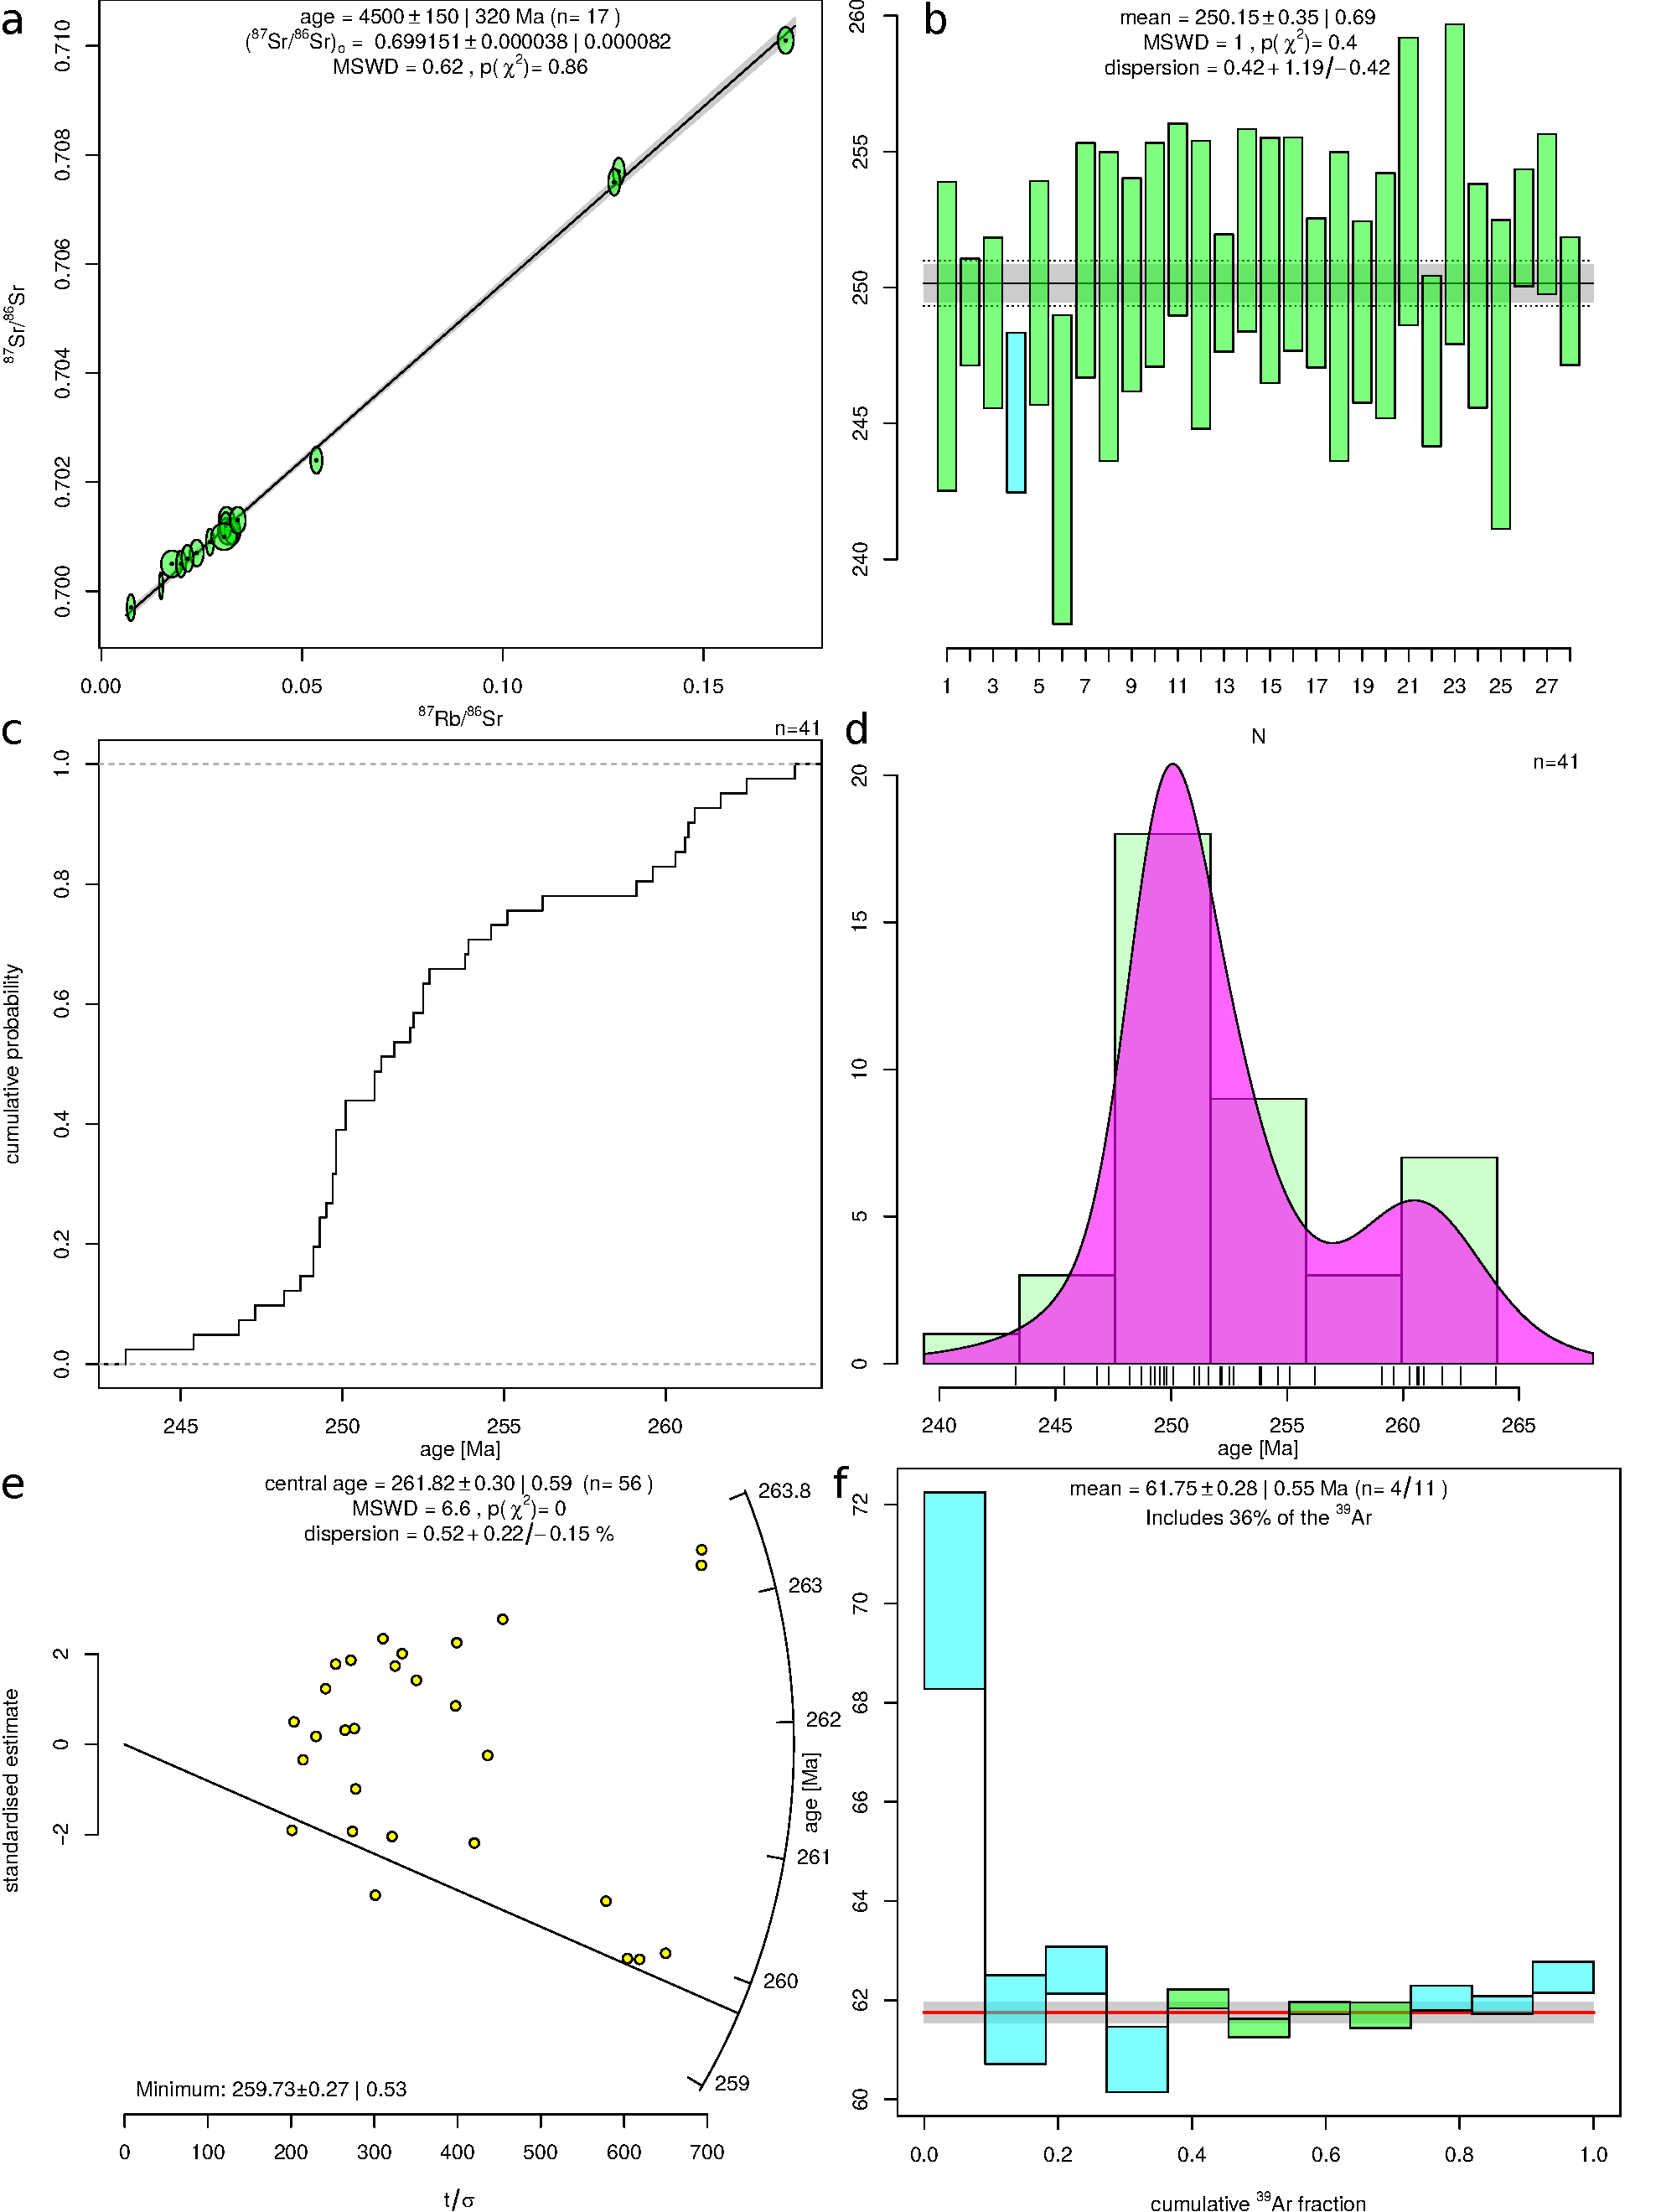
\includegraphics[width=.8\textwidth]{fig1.pdf}
  \caption{ a. `model-1' isochron of Rb-Sr data from
    \citet{compston1971}, with error ellipses and regression envelope
    shown at 95\% confidence and uncertainties stated as `$x~|~y$'
    where $x$ stands for the standard error and $y$ for the
    studentised 95\% confidence interval; b. weighted mean of
    synthetic U-Pb data from \citet{ludwig2003}, with the 95\%
    confidence interval shown as a grey band and the dispersion (also
    evaluated at 95\% confidence) shown as dotted lines; c. cumulative
    age distribution (CAD) of a synthetic U-Pb dataset from
    \citet{ludwig2003}; d. kernel density estimate (KDE) and histogram
    of the same dataset; e. radial plot of an artificial mixture of
    U-Pb data from \citet{ludwig2003}, with the minimum age estimate
    marked as a line and the (asymmetric) confidence limits for the
    dispersion shown at 95\% confidence; f. age spectrum of a
    \textsuperscript{40}Ar/\textsuperscript{39}Ar dataset from Skye
    provided by S. Sherlock (Open University), with plateau steps
    shown in green and the 95\% confidence interval for the weighted
    mean shown in grey. See Appendix~B for \texttt{R}-code to
    reproduce these plots.}
  \label{fig:1}
\end{figure}

\section{U-Pb and Pb-Pb}
\label{sec:UPb}

Uranium has two long-lived isotopes (\textsuperscript{238}U and
\textsuperscript{235}U) that occur at a nearly constant ratio of
137.818 $\pm$ 0.045 in igneous accessory minerals \citep{hiess2012}.
The nuclei of both isotopes undergo a chain of radioactive ($\alpha$,
$\beta$ and $\gamma$) decay events to different isotopes of
lead. \textsuperscript{238}U decays to \textsuperscript{206}Pb with a
half-life of 4.468 billion years, whereas \textsuperscript{235}U
decays to \textsuperscript{207}Pb with a half-life of 703.8 million
years \citep{jaffey1971}.\\

During its radioactive decay, uranium produces numerous short-lived
intermediate daughters that form the basis of U-series disequilibrium
dating (Section~\ref{sec:ThU}). It also produces seven (for
\textsuperscript{235}U) or eight (for \textsuperscript{238}U) helium
atoms, forming the basis of yet another geochronometer
(Section~\ref{sec:UThHe}). If a sufficiently long time ($>$ 2 million
years, say) has elapsed since isotopic closure, allowing the decay
chains to settle into a state of secular equilibrium, then the
intermediate daughters can be ignored and the
\textsuperscript{206}Pb/\textsuperscript{238}U- and
\textsuperscript{207}Pb/\textsuperscript{235}U-systems can be safely
treated like the simple parent-daughter pairs of
Section~\ref{sec:PD}.\\

The great power of the U-Pb method lies in the fact that it is based
on the simultaneous decay of two isotopes of the same radioactive
parent (U) to two isotopes of the same stable daughter (Pb).  This
provides the U-Pb clock with an internal consistency check that is
absent from most other geochronometers. This consistency check can be
visualised by plotting the
\textsuperscript{206}Pb/\textsuperscript{238}U-ratio measurements
against the
\textsuperscript{207}Pb/\textsuperscript{235}U-measurements on a
`Wetherill concordia' diagram \citep{wetherill1956}.\\

Alternatively, a `Tera-Wasserburg concordia' diagram plots the
\textsuperscript{207}Pb/\textsuperscript{206}Pb-ratios against the
\textsuperscript{238}U/\textsuperscript{206}Pb-ratios
\citep{tera1972}. The subspace of all compositions that yield
consistent ages between both clocks is called the `concordia line'.
Samples that plot on or near this line represent the gold standard in
geochronological reliability (Figure~\ref{fig:2}.a).\\

Samples that plot further away from the concordia line can do so for
several reasons: (1) the existence of an inherited non-radiogenic
component; (2) the partial loss of radiogenic lead during
metamorphism; (3) initial daughter disequilibrium; and (4) the mixture
of different growth zones of different age during isotopic
analysis. Only the first three mechanisms can be corrected for by
\emph{a posteriori} mathematical procedures \citep{mclean2011}.\\

\texttt{IsoplotR} implements six different methods to correct for the
presence of non-radiogenic (`common') lead. This includes three
strategies tailored to datasets that include \textsuperscript{204}Pb
measurements and a further three strategies for datasets that do not.
\textsuperscript{204}Pb is the only one of lead's four stable isotopes
that does not have a naturally occurring radioactive parent. This
makes it very useful for common-Pb correction:

\begin{equation}
  \left[\frac{{}^{206|7}Pb}{{}^{204}Pb}\right]_r =
  \left[\frac{{}^{206|7}Pb}{{}^{204}Pb}\right]_m -
  \left[\frac{{}^{206|7}Pb}{{}^{204}Pb}\right]_\circ
  \label{eq:common-Pb}
\end{equation}

\noindent where $[{}^{206|7}Pb/^{204}Pb]_r$ marks the radiogenic
${}^{206}$Pb or ${}^{207}$Pb component; $[{}^{206|7}Pb/^{204}Pb]_m$ is
the measured ratio; and $[{}^{206|7}Pb/^{204}Pb]_\circ$ is the
non-radiogenic component.\\

\texttt{IsoplotR} offers three different ways to determine
$[{}^{206|7}Pb/^{204}Pb]_\circ$. The first and easiest option is to
simply use a nominal value such as the
${}^{206|7}$Pb/\textsuperscript{204}Pb-ratio of a cogenetic feldspar,
assuming that this is representative for the common-Pb composition of
the entire sample \citep[e.g.,][]{chew2014}. A second method is to
determine the non-radiogenic isotope composition by fitting an
isochron line through multiple aliquots of the same sample, using the
3-dimensional regression algorithm of \citet{ludwig1998}.\\


Unfortunately, neither of these two methods is applicable to detrital
samples, which generally lack identifiable cogenetic minerals and
aliquots. For such samples, \texttt{IsoplotR} infers the common-Pb
composition from the two-stage crustal evolution model of
\citet{stacey1975}. The second stage of this model is described by:

\begin{equation}
  \left[\frac{{}^{206}Pb}{{}^{204}Pb}\right]_\circ =
  \left[\frac{{}^{206}Pb}{{}^{204}Pb}\right]_{3.7Ga} +
  \left[\frac{{}^{238}U}{{}^{204}Pb}\right]_{sk}
  \left(e^{\lambda_{238}[3.7Ga - t]}-1\right)
  \label{eq:stacey-kramers}
\end{equation}

\noindent where $\left[{}^{206}Pb/{}^{204}Pb\right]_{3.7Ga} =
11.152$ and $\left[{}^{238}U/{}^{204}Pb\right]_{sk} = 9.74$.
Equations~\ref{eq:common-Pb} and \ref{eq:stacey-kramers} can be solved
iteratively for $t$ and $\left[{}^{206}Pb/{}^{204}Pb\right]_\circ$
\citep{chew2014}. The
\textsuperscript{207}Pb/\textsuperscript{204}Pb-ratio is corrected in
exactly the same way, using
$\left[{}^{207}Pb/{}^{204}Pb\right]_{3.7Ga} = 12.998$.\\

Unfortunately, it is not always possible to measure
\textsuperscript{204}Pb, which is a rare and therefore hard to detect
nuclide, especially on single collector mass spectrometers and in the
presence of isobaric interferences such as \textsuperscript{204}Hg
that often occur in ICPMS instruments. In the absence of
\textsuperscript{204}Pb measurements, \texttt{IsoplotR} applies a
\textsuperscript{207}Pb-based common lead correction:

\begin{equation*}
  \left[\frac{{}^{207}Pb}{{}^{206}Pb}\right]_m =
  f \left[\frac{{}^{207}Pb}{{}^{206}Pb}\right]_\circ +
  (1-f) \left[\frac{{}^{207}Pb}{{}^{204}Pb}\right]_r
  %\label{eq:207-correction}
\end{equation*}

\noindent where $f$ is the fraction of common lead, and
$[{}^{207}Pb/{}^{206}Pb]_r$ is obtained by projecting the U-Pb
measurements on the concordia line in Tera-Wasserburg space.  Like
before, the initial lead composition $[{}^{207}Pb/{}^{206}Pb]_\circ$
can be obtained in three possible ways: by analysing a cogenetic
mineral, by isochron regression through multiple aliquots, or from the
\citet{stacey1975} model.\\

Besides the common-Pb problem, a second reason for U-Pb discordance is
radiogenic Pb-loss during igneous and metamorphic activity.  This
moves the data away from the concordia line along a linear array,
forming an isochron or `discordia' line.  \texttt{IsoplotR} fits this
line using the \citet{ludwig1998} algorithm. If the data are plotted
on a Wetherill concordia diagram, the program will not only report the
usual lower intercept with the concordia line, but the upper intercept
as well. Both values are geologically meaningful as they constrain
both the initial igneous age as well as the timing of the partial
resetting event.\\

Initial daughter disequilibrium is the third and final correctable
mechanism for U-Pb discordance. It occurs because the partition
coefficients for U, Th (and Pa) may differ significantly between the
magma and the dated mineral. Th-disequilibrium correction requires the
measurement of \textsuperscript{208}Th, which is not currently
accommodated by any of \texttt{IsoplotR}'s input formats. This may
change in future versions of the program. In the meanwhile, the user
is advised to apply the disequilibrium correction before entering
their data into \texttt{IsoplotR} \citep{mclean2011}.\\

The Pb-Pb method is based on the same radioactive decay scheme as the
U-Pb method but only involves the isotopic ratios of one element, Pb
(assuming that the \textsuperscript{235}U/\textsuperscript{238}U-ratio
is independently known):

\begin{equation*}
  \left[\frac{{}^{207}Pb}{{}^{206}Pb}\right]_r =
  \left[\frac{{}^{235}U}{{}^{238}U}\right]
  \frac{e{}^{\lambda_{235}t}-1}{e{}^{\lambda_{238}t}-1}
  %\label{eq:PbPb}
\end{equation*}

In this respect the Pb-Pb method is similar to the
\textsuperscript{40}Ar/\textsuperscript{39}Ar-method.  This similarity
extends to the construction of isochrons which, like for the
\textsuperscript{40}Ar/\textsuperscript{39}Ar-method, come in two
forms. The `normal' isochron plots the
\textsuperscript{207}Pb/\textsuperscript{204}Pb-ratio against the
\textsuperscript{206}Pb/\textsuperscript{204}Pb-ratio, the slope of
which yields the radiogenic
\textsuperscript{207}Pb/\textsuperscript{206}Pb-ratio.\\

The `inverse' isochron plots the
\textsuperscript{207}Pb/\textsuperscript{206}Pb-ratio against the
\textsuperscript{204}Pb/\textsuperscript{206}Pb-ratio, yielding the
radiogenic \textsuperscript{207}Pb/\textsuperscript{206}Pb-ratio as
the intercept. Again, the error correlations are smaller for the
inverse isochron than they are for the conventional one
\citep{connelly2017}.

\section{\textsuperscript{230}Th-U}
\label{sec:ThU}

\textsuperscript{238}U and \textsuperscript{206}Pb are part of a decay
chain that comprises seven intermediate daughters. The half lives of
all these daughters are more than four orders of magnitude shorted
than that of \textsuperscript{238}U, with \textsuperscript{234}U
($t_{1/2} = 246$~ka) and \textsuperscript{230}Th ($t_{1/2} = 76$~ka)
being the least radioactive among them \citep{cheng2013}.\\

Samples whose age exceeds $\sim$2~Ma enter a state of secular
equilibrium whereby the \textsuperscript{234}U/\textsuperscript{238}U-
and \textsuperscript{230}Th/\textsuperscript{238}U-activity ratios
approach unity. Such samples are amenable to U-Pb dating as described
in Section~\ref{sec:UPb}. For younger samples, the degree to which an
initially disrupted \textsuperscript{238}U-decay chain has restored
secular equilibrium forms the basis of a separate class of
geochronometers that are collectively referred to as U-series
dating.\\

U and Th have contrasting chemical properties and are easily
fractionated during chemical processes such as crystallisation. This
fractionation disrupts any pre-existing state of secular equilibrium
between \textsuperscript{230}Th and its parent nuclide
\textsuperscript{234}U. Additionally, the secular equilibrium between
\textsuperscript{234}U and its parent \textsuperscript{238}U may be
disturbed by the physical processes of alpha-recoil, which can
dislodge \textsuperscript{234}U from the original
\textsuperscript{238}U site \citep{moore1967}.\\

The first mechanism occurs in young volcanic rocks, which are often
enriched (and occasionally depleted) in Th relative to U with respect
to the magma from which they were derived, but whose
\textsuperscript{234}U/\textsuperscript{238}U-ratio remains in secular
equilibrium. In contrast with this, carbonates can be out of
equilibrium in both their
\textsuperscript{230}Th/\textsuperscript{234}U- and
\textsuperscript{234}U/\textsuperscript{238}U-activity ratios, due to
the low solubility of Th in water and the enrichment of
\textsuperscript{234}U relative to \textsuperscript{238}U in rivers,
lakes, seas, caves and other geologic environments. In this general
case, the evolution of the
\textsuperscript{230}Th-\textsuperscript{234}U-\textsuperscript{238}U-system
with time is described by:

\begin{equation}
  \frac{A[{}^{230}Th] - A[{}^{230}Th]_\circ}{A[{}^{238}U]} =
  1 - e^{\lambda_{230}t} -
  \left(\frac{A[{}^{234}U]}{A[{}^{238}U]}-1\right)
  \left(\frac{\lambda_{230}}{\lambda_{234}-\lambda_{230}}\right)
  \left(1-e^{[\lambda_{234}-\lambda_{230}]t}\right)
  \label{eq:Th-U}
\end{equation}

\noindent where $A[\ast]$ is the activity of $\ast$ and
$A[{}^{230}Th]_\circ$ is the `detrital' \textsuperscript{230}Th
component, i.e. the \textsuperscript{230}Th that was already present
in the sample at the time of its formation \citep{kaufman1965,
  ludwig2003b}. This component is unknown but can be estimated by
isochron regression using long-lived \textsuperscript{232}Th as a
normalising factor.\\

For igneous samples, in which $A[{}^{234}U]/A[{}^{238}U] = 1$, the
second term on the right-hand side of Equation~\ref{eq:Th-U} vanishes
and we can write:

\begin{equation}
  \left(\frac{A[{}^{230}Th]}{A[{}^{232}Th]}\right)_i = 
  \left(\frac{A[{}^{230}Th]}{A[{}^{232}Th]}\right)_\circ +
  \left(\frac{A[{}^{238}U]}{A[{}^{232}Th]}\right)_i
  \left(1-e^{-\lambda_{230}t}\right)
  \label{eq:Th-U-volcanic}
\end{equation}

\noindent for $1 \leq i \leq n$, which can be solved for $t$ and
$\left(A[{}^{230}Th]/A[{}^{232}Th]\right)_\circ$ using the least
squares method of \citet{york2004}. Equation~\ref{eq:Th-U-volcanic}
forms a `Rosholt'-type isochron, which is akin to a `normal' isochron
in Rb-Sr or Ar-Ar geochronology \citep{rosholt1976}. Using
$A[{}^{238}U]$ as the normalising factor instead yields an
`Osmond'-type isochron, which is akin to an `inverse' isochron in
Ar-Ar or Pb-Pb geochronology \citep{osmond1970, ludwig2003b}.\\

For carbonate samples, in which \textsuperscript{234}U and
\textsuperscript{238}U generally are not in secular equilibrium, three
activity ratios are needed to determine the detrital
\textsuperscript{230}Th (and initial \textsuperscript{234}U)
component. This in turn requires three dimensional isochron regression
of the \textsuperscript{230}Th/\textsuperscript{238}U-,
\textsuperscript{232}Th/\textsuperscript{238}U- and
\textsuperscript{234}U/\textsuperscript{238}U-activity
ratios. \texttt{IsoplotR} performs this calculation with the maximum
likelihood algorithm of \citet{ludwig1994}.\\

In addition to (Rosholt and Osmond) isochrons and the usual weighted
mean, radial, CAD and KDE plots, U-series data can also be visualised
on Th-U evolution diagrams.  For carbonate data, these consist of a
scatter plot that sets out the
\textsuperscript{234}U/\textsuperscript{238}U-activity ratios against
the \textsuperscript{230}Th/\textsuperscript{238}U-activity ratios as
error ellipses, and displays the initial
\textsuperscript{234}U/\textsuperscript{238}U-activity ratios and ages
as a set of intersecting lines (Figure~\ref{fig:2}.b).\\

The Th-U evolution diagram has a similar purpose and appearance as the
U-Pb concordia diagram, which also displays compositions and dates
simultaneously. An alternative way of doing so for carbonate samples
is by plotting the initial
\textsuperscript{234}U/\textsuperscript{238}U-ratios against the
\textsuperscript{230}Th-\textsuperscript{234}U-\textsuperscript{238}U-ages
(Figure~\ref{fig:2}.c).  In both types of evolution diagrams,
\texttt{IsoplotR} provides the option to project the raw measurements
along the best fitting isochron line and thereby remove the detrital
\textsuperscript{230}Th-component. This procedure allows a visual
assessment of the degree of homogeneity within a dataset, as is
quantified by the MSWD.\\

Neither the U-series evolution diagram nor the
\textsuperscript{234}U/\textsuperscript{238}U vs. age plot is
applicable to igneous datasets, in which \textsuperscript{234}U and
\textsuperscript{238}U are in secular equilibrium.  For such datasets,
\texttt{IsoplotR} produces an Osmond-style regression plot that is
decorated with a fanning set of isochron lines.

\section{U-Th-(Sm)-He}
\label{sec:UThHe}

The radioactive decay of uranium produces not only lead
(Section~\ref{sec:UPb}) and short-lived \textsuperscript{234}U and
\textsuperscript{230}Th (Section~\ref{sec:ThU}), but seven (for
\textsuperscript{235}U) or eight (for \textsuperscript{238}U)
$\alpha$-particles as well.  When these $\alpha$-particles acquire
electrons, they turn into helium atoms, forming the basis of yet
another geological clock. $\alpha$-decay of \textsuperscript{232}Th
and \textsuperscript{147}Sm provides additional sources of radiogenic
helium.  The ingrowth of helium with time is thus described by:

\begin{equation}
  \begin{split}
  {}^{4}He = 8 \left(e^{\lambda_{238}t} -1\right)[{}^{238}U] +
       7 \left(e^{\lambda_{235}t} -1\right)[{}^{235}U] + \\
  6 \left(e^{\lambda_{232}t} -1\right) [{}^{232}Th] +
  \left(e^{\lambda_{247}t} -1 \right) [{}^{147}Sm]
  \end{split}
  \label{eq:UThHe}
\end{equation}

Because Sm (1) produces only one $\alpha$-particle per decay event;
(2) has a very long half-life; and (3) its radioactive isotope 147
only accounts for 14.99\% of total samarium, Sm can be ignored as a
parent in all but the most Sm-rich samples. For this reason, some
laboratories do not measure Sm at all and hence we will refer to the
helium dating method as the `U-Th-(Sm)-He' method in the remainder of
this text.\\

Equation~\ref{eq:UThHe} can be solved for $t$ iteratively. Like argon,
helium is a noble gas that is lost to the environment (and eventually
to space) at high temperatures by volume diffusion.  Additional
complication is added by the physical separation of the parent and
daughter nuclides in the U-Th-(Sm)-He system. This separation results
from the energy released during $\alpha$-decay, which displaces the
$\alpha$-particles by up to \SI{16}{\micro\metre} and may result in
the ejection of helium produced by parent atoms that are sited near
the edges of the host mineral \citep{farley1996}. That lost helium
must be taken into account when interpreting the thermal history of a
sample \citep{meesters2002b}. For rapidly cooled samples, this can be
done by applying a geometric correction to the U, Th and
Sm-measurements \citep{ketcham2011}.  \texttt{IsoplotR} assumes that
such an `$\alpha$-ejection correction' has been applied to the data
prior to age calculation.\\

More often than not, and more often than for other geochronometers,
U-Th-(Sm)-He data are overdispersed with respect to the analytical
uncertainties \citep{fitzgerald2006}. Several mechanisms have been
invoked to explain this overdispersion, including compositional
effects \citep{djimbi2015}, radiation damage \citep{flowers2009,
  guenthner2013}, and breakage during mineral separation
\citep{brown2013}.\\

\texttt{IsoplotR} implements four different ways to visualise and
quantify the overdispersion.  The first two of these are the weighted
mean and radial plot, which were discussed in
Sections~\ref{sec:averaging} and \ref{sec:density}. The third way is
the isochron plot and age. This uses a first order approximation of
the U-Th-(Sm)-He age equation:

\begin{equation}
  t \approx \left[{}^{4}He\right]/\left\{
    8\lambda_{238}[{}^{238}U] + 7\lambda_{235}[{}^{235}U] +
    6\lambda_{232} [{}^{232}Th] + \lambda_{147} [{}^{147}Sm]
    \right\}
  \label{eq:t=HeP}
\end{equation}

\noindent which is accurate to better than \SI{1}{\percent} for ages
less than 100~Ma \citep{vermeesch2008a}. A U-Th-(Sm)-He isochron is
constructed by plotting the numerator of the right-hand side of
Equation~\ref{eq:t=HeP} against the denominator and fitting a straight
line through several aliquots of the same sample. Because the parent
and daughter nuclides are analysed separately on different mass
spectrometers, their uncertainties are uncorrelated with each
other. Therefore, the isochron regression can be done using the simple
least squares fitting method of \citet{york1966}.\\

The fourth and final way to visualise and average U-Th-(Sm)-He data is
based on the fact that U, Th, Sm and He are \emph{compositional}
data. This means that it is not so much the absolute concentrations of
these elements that bear the chronological information, but rather
their relative proportions. Equation~\ref{eq:UThHe} can be recast in
terms of the elemental ratios U/He, Th/He and Sm/He, which take on
strictly positive values.  The space of all possible U-Th-He
compositions fits within the constraints of a ternary diagram or
`helioplot' \citep{vermeesch2010a}. If Sm is included as well, then
this expands to a three-dimensional tetrahedral space
\citep{vermeesch2008a}.\\

Conventional statistical analysis of data that fit within these
constrained spaces is fraught with theoretical and practical
problems. For example, the arithmetic mean of compositional data may
yield meaningless values, and their `2-sigma' confidence bounds may
include physically impossible negative values \citep[Figures~3 and 5
  of][]{vermeesch2006b}.\\

Geologists had been aware of these problems for many decades
\citep[e.g.,][]{chayes1956}.  But it was not until the 1980s that a
solution was found to the compositional data conundrum, when
\citet{aitchison1982,aitchison1986} showed that all the problems
caused by the constant sum constraint can be solved by applying a
simple logratio transformation.  This idea is similar to the
log-transformation that was used for the mixture models of
Section~\ref{sec:mixtures}. In the case of the U-Th-He-(Sm)-He system,
the logratio analysis is achieved by first defining two (or three) new
variables:

\begin{equation*}
  u \equiv \ln\left[U\big/He\right],
  v \equiv \ln\left[Th\big/He\right]
  \left(, w \equiv \ln\left[Sm\big/He\right] \right)
\end{equation*}

\noindent and then performing the desired statistical analysis
(averaging, uncertainty propagation, ...) on the transformed data
\citep{vermeesch2008a,vermeesch2010a,vermeesch2015b}. Upon completion
of the mathematical operations, the results can then be mapped back to
U-Th-(Sm)-He space using an inverse logratio transformation:

\begin{equation*}
  \begin{array}{l@{}r@{}l}
    [He] = 1\big/\left[e^{u}+e^{v}+(e^{w})+1\right]
    &,~&
    [U] = e^{u}\big/\left[e^{u}+e^{v}+(e^{w})+1\right], \\~
    [Th] = e^{v}\big/\left[e^{u}+e^{v}+(e^{w})+1\right]
    &\big(,~&
    [Sm] = e^{w}\big/\left[e^{u}+e^{v}+(e^{w})+1\right] \big)
  \end{array}
\end{equation*}

\noindent where $[He] + [U] + [Th] (+ [Sm]) = 1$. In the context of
U-Th-(Sm)-He dating, the central age is defined as the age that
corresponds to the arithmetic mean composition in logratio space,
which is equivalent to the geometric mean in compositional dataspace
\citep{vermeesch2008a}. \texttt{IsoplotR}'s \texttt{helioplot}
function performs this calculation using the same algorithm that is
used to obtain the weighted mean U-Pb composition for the concordia
age calculation (Section~\ref{sec:UPb}).\\

Overdispersion is treated similarly as in a regression context
(Section~\ref{sec:regression}).  Thus, there are options to augment
the uncertainties with a factor $\sqrt{MSWD}$ (model-1); to ignore the
analytical uncertainties altogether (model-2); or to add a constant
overdispersion term to the analytical uncertainties (model-3).  The
\texttt{helioplot} function visualises U-Th-(Sm)-He data on either a
ternary diagram or a bivariate $\ln[Th/U]$ vs. $\ln[U/He]$ contour
plot (Figures~\ref{fig:2}.d and e). These diagrams provide a
convenient way to simultaneously display the isotopic composition of
samples and their chronological meaning. In this respect, they fulfil
the same purpose as the U-Pb concordia diagram and the U-series
evolution plot.

\section{Fission tracks}
\label{sec:FT}

\textsuperscript{238}U is the heaviest naturally occurring nuclide in
the Solar System, and the only one that undergoes spontaneous fission.
On average only 1 spontaneous fission event occurs for every 1.8
million $\alpha$-decay events \citep{holden2000}, and so the number of
fission tracks that accumulate over geologic time is small enough to
be counted by a human observer, using a petrographic microscope. The
fission track age is then given by:

\begin{equation}
  t = \frac{1}{\lambda_{238}}
  \ln\left(
  1 + \frac{\lambda_{238}}{\lambda_f}\frac{2 N_s}{[{}^{238}U]A_sL}
  \right)
  \label{eq:FT}
\end{equation}

\noindent where $N_s$ is the number of spontaneous fission tracks
measured over an area $A_s$, $[{}^{238}U]$ is the
\textsuperscript{238}U-concentration in atoms per unit volume,
$\lambda_f$ is the fission decay constant \citep[$8.5 \times
  {10}^{-17}$ yr\textsuperscript{-1},][]{holden2000}, $L$ is the
etchable fission track length, and the factor 2 is a geometric factor
accounting for the fact that etching reveals tracks from both above
and below the internal crystal surface.\\

Two analytical approaches are used to measure $[{}^{238}U]$: neutron
activation and LAICPMS. The first approach estimates the
\textsuperscript{238}U-concentration indirectly, using the induced
fission of neutron-irradiated \textsuperscript{235}U as a proxy for
the \textsuperscript{238}U. In the most common implementation of this
approach, the induced fission tracks are recorded by an external
detector made of mica or plastic that is attached to the polished
grain surface \citep{fleischer1972, hurford1983}. The fission track
age equation then becomes:

\begin{equation*}
  t = \frac{1}{\lambda_{238}}
  \ln\left(
  1 + \frac{\lambda_{238}\zeta\rho_d}{2}\frac{N_s}{N_i}
  \right)
%  \label{eq:EDM}
\end{equation*}

\noindent where $N_i$ is the number of induced fission tracks counted
in the external detector over the same area as the spontaneous tracks,
$\zeta$ is a `zeta'-calibration factor that incorporates both the
fission decay constant and the etchable fission track length, and
$\rho_d$ is the number of induced fission tracks per unit area counted
in a co-irradiated glass of known U-concentration. $\rho_d$ allows the
$\zeta$-factor to be `recycled' between irradiations. The appeal of
the external detector method (EDM) lies in the fact that it imposes a
`paired experimental design' on the fission track method, which makes
it insensitive to uranium zoning, and greatly simplifies subsequent
statistical analysis \citep{galbraith2010b}.\\

Despite the elegance of the EDM, a growing number of laboratories are
adopting LAICPMS as an alternative means of determining the
\textsuperscript{238}U-content of fission track samples
\citep{hasebe2004, chew2012}. The main reasons for this change are the
increased throughput achieved by not having to irradiate samples and
the ease of double-dating apatite and zircon with the U-Pb
method. Unfortunately, abandoning the EDM in favour of LAICPMS also
removes the paired experimental design and causes problems in dealing
with U-zoning an zero-track grains. \citet{vermeesch2017} proposes
four different strategies to deal with these problems, all of which
are implemented in \texttt{IsoplotR}.\\

A first option is to only count the spontaneous fission tracks that
are located within the laser ablation spot, and to plug the resulting
track counts, areas and \textsuperscript{238}U-concentrations into
Equation \ref{eq:FT}.  Matching the areas over which $N_s$ and
$[{}^{238}U]$ are measured reduces the detrimental effect of (lateral)
U-zoning on the fission track age accuracy. The main limitation of
matching the areas is a reduction in precision due to the low number
of spontaneous tracks counted within the outline of a small ablation
pit. This problem can be circumvented by acquiring multiple
\textsuperscript{238}U-measurements per grain.\\

In a second approach to LAICPMS-based fission track dating,
\texttt{IsoplotR} then jointly considers all the grains that have been
analysed multiple times to quantify the degree of U-zoning within the
grains.\\

The accuracy of the two `absolute dating' approaches discussed thus
far is fundamentally limited by the accuracy of the U-concentration
measurements, the fission track decay constant and the etching and
counting efficiencies.  Unfortunately, all these factors are
potentially affected by unquantifiable biases.\\

The third (using a single laser spot per grain) and fourth (using
multiple spots) approach to LAICPMS-based fission track dating remove
these systematic errors by normalising to a standard of known fission
track age and defining a new `zeta' calibration constant
$\zeta_{icp}$:

\begin{equation}
  t = \frac{1}{\lambda_{238}} \ln\left( 1 +
  \frac{\lambda_{238}\zeta_{icp}}{2} \frac{N_s}{[{}^{238}U] A_s} \right)
  \label{eq:tICPzeta}
\end{equation}

\noindent where $[{}^{238}U]$ may either stand for the
\textsuperscript{238}U-concentration (in ppm) \emph{or} for the U/Ca
(for apatite) or U/Si (for zircon) ratio measurement, and $A_s$ is the
spontaneous track counting area.  \texttt{IsoplotR} implements the
four approaches to LAICPMS-based fission track dating by giving the
user the choice between an `absolute' and `$\zeta$-calibration'
option, and between one or more U-measurements per grain.\\

The zero track problem is solved by converting the U-concentration
measurements into a `virtual' induced track density ($\hat{N}_i$) by
replacing $[{}^{238}U] A_s$ with $\hat{N}_i/\rho_{icp}$ in
Equation~\ref{eq:tICPzeta}, so that the Poisson uncertainty of
$\hat{N}_i$ matches the uncertainty of the U-concentration measurement
\citep{vermeesch2017}.

\section{Detrital geochronology}
\label{sec:detritals}

The principal aim of the methods and graphical devices discussed thus
far has been to extract geologically meaningful information from
multiple aliquots of a single sample. However, most geochronological
applications nowadays involve multiple samples, and the differences
between these samples often has greater scientific significance than
any individual date.  \texttt{IsoplotR} implements a number of
graphical devices to facilitate the interpretation of such
multi-sample datasets.\\

As was discussed in Section~\ref{sec:density}, the CAD is the easiest
way to simultaneously visualise multiple age distributions on a single
plot. In contrast, KDEs are better presented in a multi-panel
format. To facilitate the intercomparison of multiple age
distributions, \texttt{IsoplotR} offers the option to force all panels
to use the same kernel bandwidth, to normalise the area under each KDE
to a common value, and to plot them all on the same timescale.\\

Visual comparison of CADs or KDEs can be an effective way to spot
general trends and groupings in simple datasets. But this approach
becomes impractical when the inter-sample differences are subtle or
the datasets are large ($> 10$ samples, say). Such cases call for an
additional layer of statistical simplification to emphasise the
geologically significant differences whilst removing the less
informative similarities. Multi-dimensional scaling (MDS) is one way
to achieve this goal.\\

MDS is a dimension-reducting technique that takes a matrix of pairwise
`dissimilarities' between objects (in our case age distributions) as
input and produces a `map' as output, on which similar samples cluster
closely together and dissimilar samples plot far apart
(Figure~\ref{fig:2}.f). In the context of detrital geochronology, the
dissimilarity between samples is given by the statistical distance
between age distributions. There are many ways to define this
statistical distance \citep{vermeesch2018b}. \texttt{IsoplotR} uses
the Kolmogorov-Smirnov (KS) statistic due to its simplicity and the
fact that it behaves like a true distance in the mathematical sense of
the word \citep{vermeesch2013, vermeesch2018b}.\\

The KS-distance is closely related to the CAD-plot that was discussed
in Section~\ref{sec:density}.  It is given by the maximum vertical
difference between two CAD step functions.  Calculating the
KS-distance between samples two at a time populates a symmetric
dissimilarity matrix with positive values and a zero
diagonal. \texttt{IsoplotR} implements two algorithms to convert this
matrix into an MDS configuration. The first (`classical' or `metric')
approach uses a sequence of basic matrix manipulations developed by
\citet{young1938} and \citet{torgerson1952} to achieve a linear fit
between the KS-distances and the fitted distances in the MDS
configuration. The second, more sophisticated (`nonmetric') approach
subjects the input distances to a transformation $f$ prior to fitting
a configuration:

\[
\delta_{i,j} = f(KS_{ij})
\]

\noindent where $KS_{i,j}$ is the KS-distance between samples $i$ and
$j$ (for $1 \leq i \neq j \leq n$) and $\delta_{i,j}$ is the
`disparity' \citep{kruskal1978}.  Fitting an MDS configuration then
involves finding the disparity transformation that maximises the
goodness of fit (or minimises the `stress') between the disparities
and the fitted distances. The latter two quantities can also be
plotted against each other as a `Shepard plot'. Additional options and
higher order alternatives to these MDS algorithms are provided in a
separate \texttt{R}-package called \texttt{provenance}
\citep{vermeesch2016a}.

\begin{figure}[p]
  \centering
  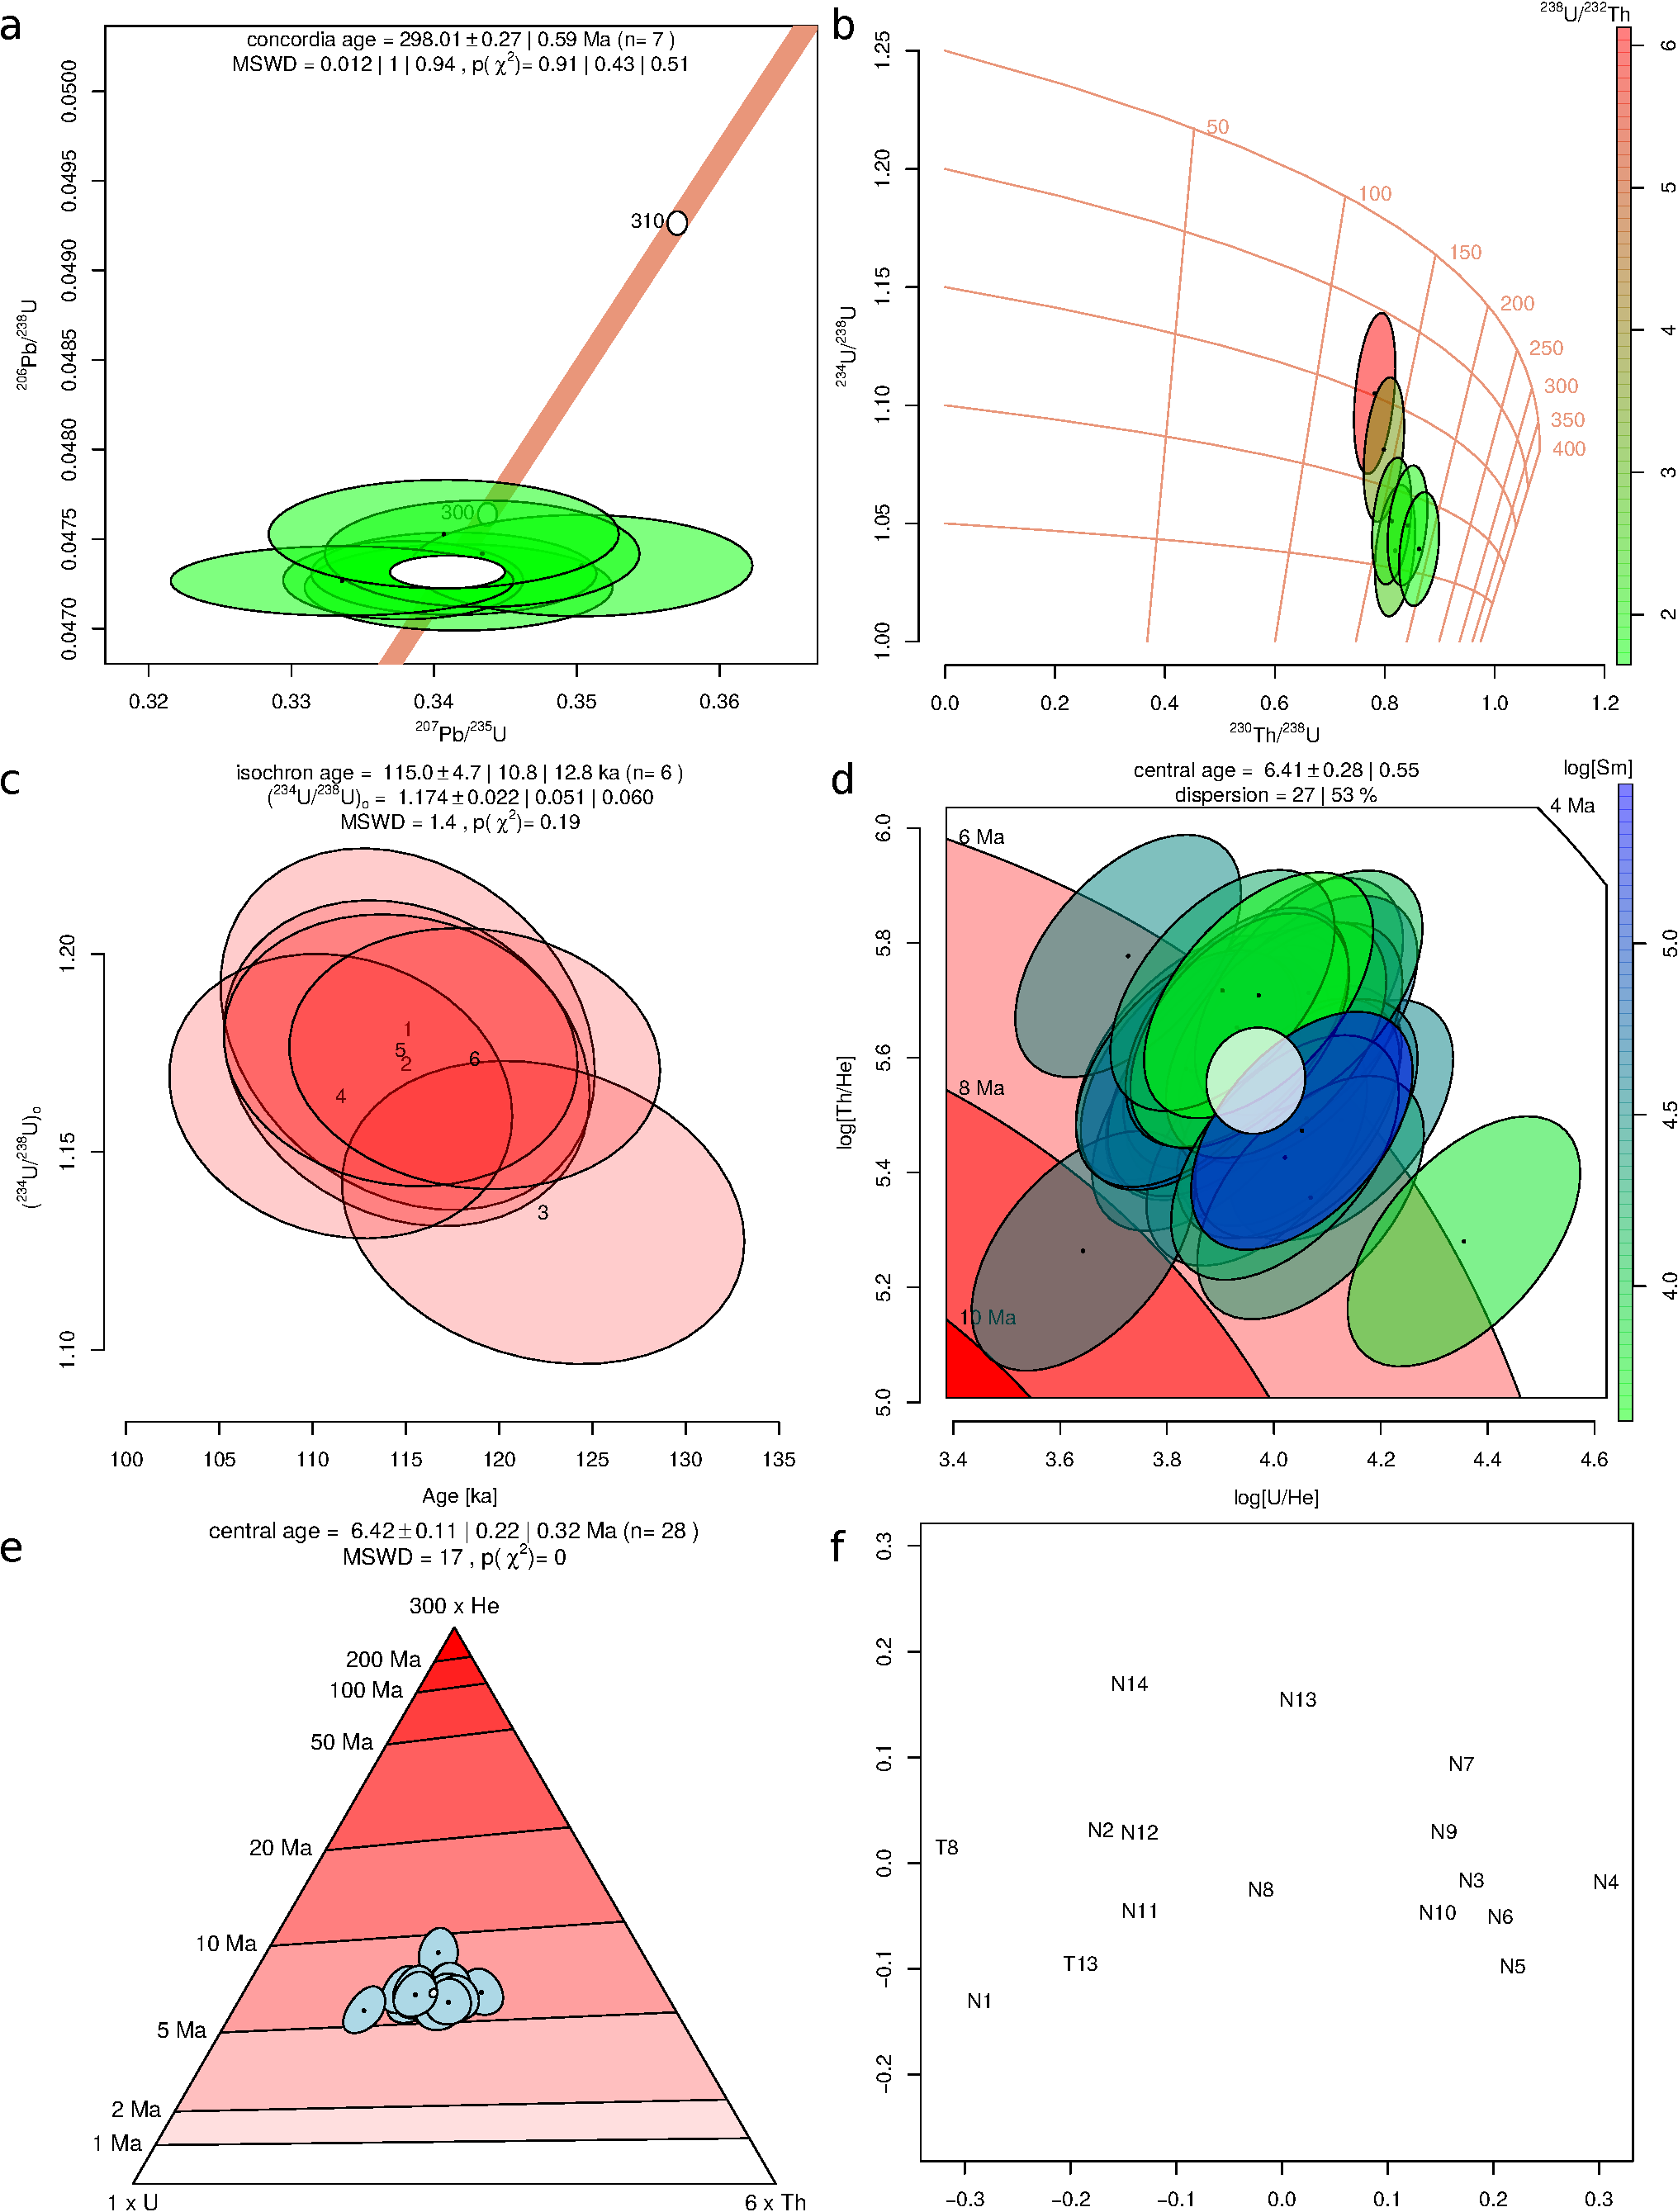
\includegraphics[width=.75\textwidth]{fig2.pdf}
  \caption{ a. Wetherill concordia diagram of U-Pb data from
    \citet{ludwig2003} that were common-Pb corrected using an isochron
    intercept obtained with the regression algorithm of
    \citet{ludwig1998}, including decay constant uncertainties; the
    three MSWD- and p-values quantify the goodness-of-fit for
    equivalence, for concordance and for their combination;
    b. \textsuperscript{230}Th-U evolution diagram of example data
    from \citet{ludwig1994}, with the
    \textsuperscript{238}U/\textsuperscript{232}Th-ratios shown as
    fill colours for the 95\% confidence ellipses; c. the same
    \textsuperscript{230}Th-U data projected along the isochron line
    on the initial \textsuperscript{234}U/\textsuperscript{238}U vs.
    \textsuperscript{230}Th-U age plane; d. U-Th-Sm-He data of
    \citet{vermeesch2008a} shown on a logratio plot with the
    Sm-content ($\log_{10}[Sm]$) represented by colours and the
    central age and composition (white ellipse) calculated from a
    `model-3' type fit; e. the same U-Th-Sm-He data shown on a ternary
    diagram, with the central age computed using a `model-1' type fit,
    and results shown as `$t~\pm~x~|~y~|~z$', where $x$ and $y$ are as
    in Figure~\ref{fig:1}.a and $z$ represents the studentised 95\%
    confidence interval augmented by a factor $\sqrt{MSWD}$;
    f. non-metric multidimensional scaling (MDS) configuration of a
    detrital zircon U-Pb dataset from \citet{vermeesch2015}. See
    Appendix~B for the \texttt{R} code corresponding to these plots.}
  \label{fig:2}
\end{figure}

\section{Future developments}
\label{sec:future}

\texttt{IsoplotR} is, and always will be, a work in progress. The
program will continue to evolve because geochronology itself continues
to evolve.  Future additions may include techniques such as K-Ar,
K-Ca, luminescence- and cosmogenic nuclide dating.  New approaches to
existing methods, such as LAICPMS-based fission track dating or
in-situ U-Th-He geochronology may prompt the addition of new input
formats or novel approaches to data visualisation. Additional user
interfaces are planned to facilitate the integration of
\texttt{IsoplotR} with existing workflows in other programming
environments. One example of this is the planned development of an
\texttt{IsoplotR4Excel} add-in that will aim to provide the same user
experience as K. Ludwig's original \texttt{Isoplot} program.

As was discussed in Section~\ref{sec:input}, rigorous error
propagation requires statistical models that keep track of the error
correlations between isotopic ratio measurements. The regression
algorithms of \citet{york1969}, \citet{ludwig1994} and
\citet{ludwig1998} take into account the covariant data structure that
is embedded \emph{within} each aliquot of a multi-aliquot set of mass
spectrometer measurements. But they do not take into account the
uncertainty correlations that may exist \emph{between} aliquots.
These correlations can be very significant due to the detector
calibrations and fractionation factors that are shared by all
measurements made on the same instrument.\\

For example, \citet{vermeesch2015b} showed that error correlations
between subsequent heating steps within a
\textsuperscript{40}Ar/\textsuperscript{39}Ar-age spectrum can be as
high as $\rho > 0.9$. Ignoring these correlations when calculating
isochrons or weighted means results in imprecise and potentially
inaccurate dates. The mathematical solution to this problem is fairly
straightforward. \citet{ludwig1998}'s maximum likelihood approach to
U-Pb isochron regression with decay constant uncertainties can serve
as a template for a generalised approach to linear regression and
averaging.\\

This approach would require a new class of input formats in which all
the isotopic ratio measurements are assembled into one large
covariance structure along with all the parameters and calibration
constants. Similar methods have already been implemented in lower
level data acquisition and processing software such as
\texttt{Ar-Ar\_Redux} \citep{vermeesch2015b} and
\texttt{U-Pb\_Redux}/\texttt{ET\_Redux} \citep{bowring2011,
  mclean2016}. At the moment there is a disconnect between these
programs and \texttt{IsoplotR}. Fortunately, both
\texttt{Ar-Ar\_Redux} and \texttt{U-Pb\_Redux}/\texttt{ET\_Redux} are
open source software. It is therefore possible to extend their code
base with functions to export processed data in a format that can be
imported into \texttt{IsoplotR}.

\section*{Acknowledgments}

The author would like to thank Chris Spencer and Noah McLean for
exceptionally insightful reviews which greatly improved the manuscript
and software.  This work was not funded. The author would like to
thank his family for their patience during the many evening and
weekend hours spent on the development of \texttt{IsoplotR}.

\clearpage

\renewcommand\thefigure{A.\arabic{figure}}    
\setcounter{figure}{0}
\section*{Appendix A: the graphical user interface (GUI)}

The GUI can either be accessed online or installed offline following
instructions that can be found on
\texttt{http://isoplotr.london-geochron.com}.

\begin{figure}[!ht]
  \centering
  \frame{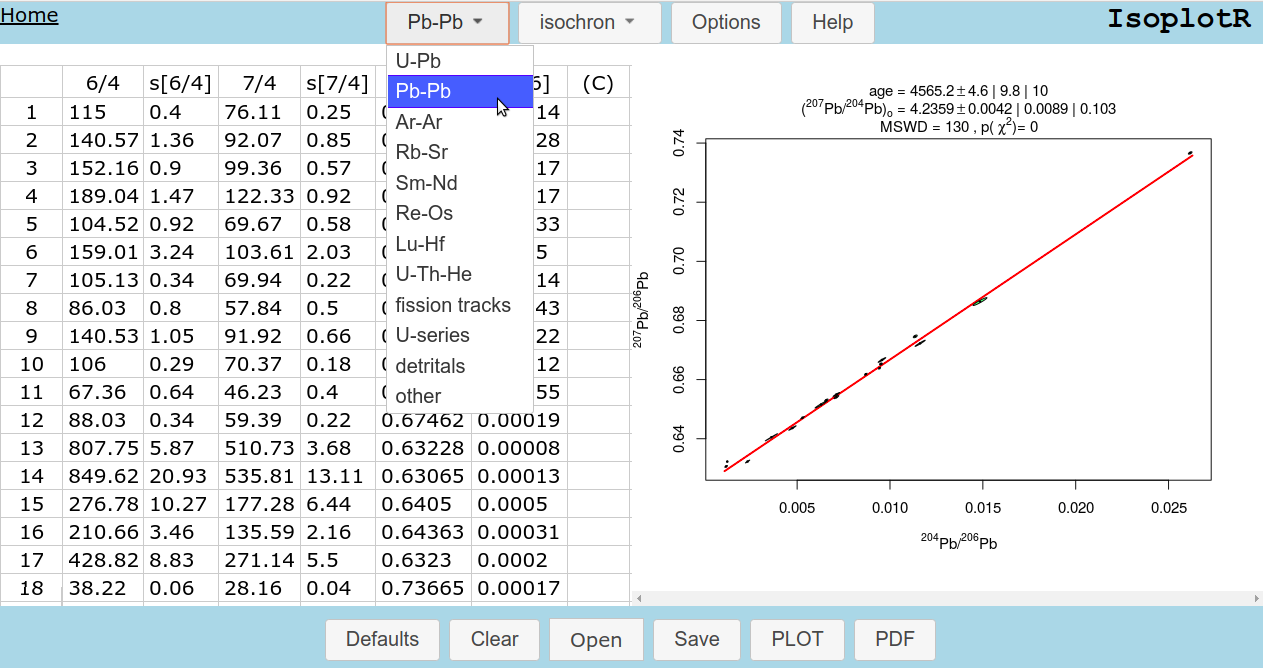
\includegraphics[width=\textwidth]{IsoplotR.png}}
  \label{fig:GUI}
  \caption{The GUI has four components: a top bar with selection menus
    for the various chronometers and plot devices, optional settings
    and documentation; an input table into which data can be pasted
    from spreadsheet applications; an output window displaying the
    graphical or numerical results; and a lower bar to import and
    export data and results.}
\end{figure}

\begin{figure}[!ht]
  \centering
  \frame{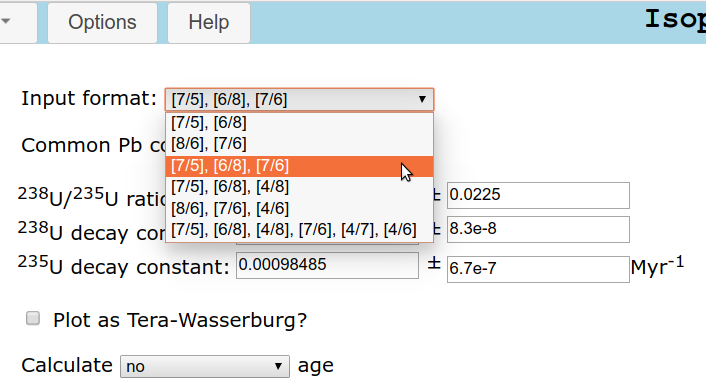
\includegraphics[width=7cm]{InputFormats.png}}
  \label{fig:input}
  \caption{Alternative input formats (shown here for the U-Pb method)
    are available through the \texttt{Options} menu.}
\end{figure}

\begin{figure}[!ht]
  \centering
  \frame{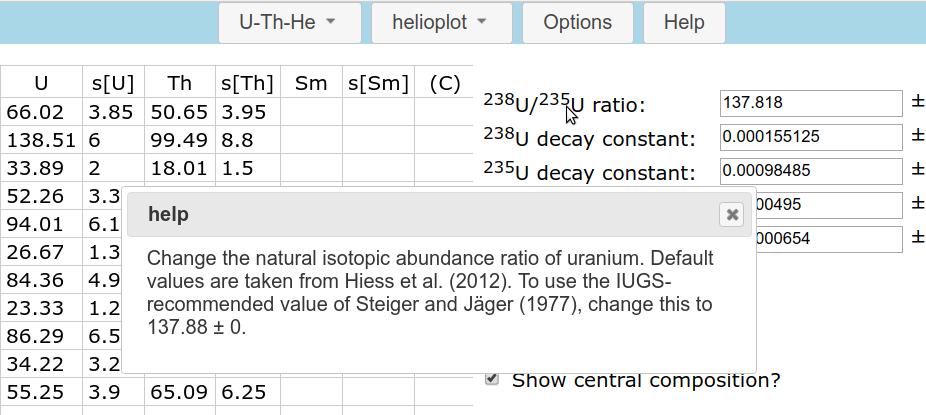
\includegraphics[width=9cm]{ContextualHelp.png}}
  \label{fig:contextualhelp}
  \caption{Contextual help (shown here for U-Th-He data) can be
    accessed by clicking on any text within the \texttt{Options}
    menu.}
\end{figure}

\begin{figure}[!ht]
  \centering
  \frame{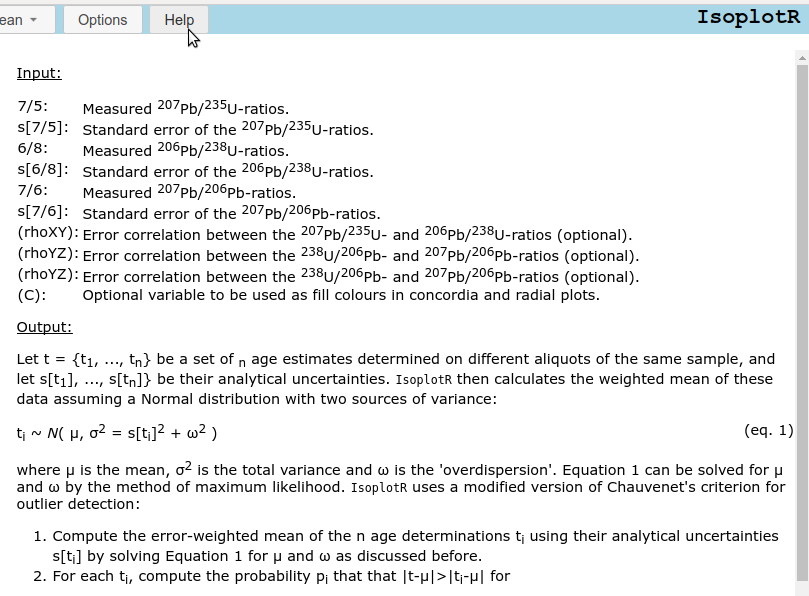
\includegraphics[width=9cm]{Help.png}}
  \label{fig:help}
  \caption{Further documentation (shown here for the weighted mean of
    U-Pb data) is provided under the \texttt{Help} menu. This includes
    information about the input and output parameters, and a brief
    summary of the theoretical background with essential references.}
\end{figure}

\begin{figure}[!ht]
  \centering
  \frame{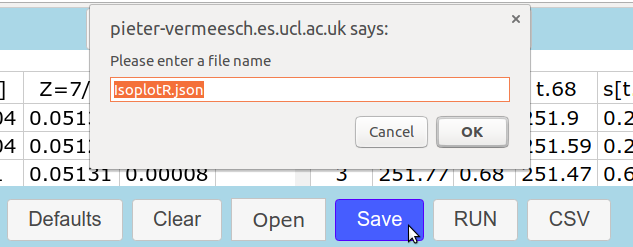
\includegraphics[width=7cm]{json.png}}
  \label{fig:json}
  \caption{Data and settings can be saved in a \texttt{.json} database
    format for future use.}
\end{figure}

\clearpage

\section*{Appendix B: command-line functionality}

Running the following commands at the \texttt{R} command prompt
reproduces all the figures in this paper. Everything that follows the
hashtag (`\#') is a comment and is ignored during execution:

\begin{verbatim}
# load the IsoplotR package:
library(IsoplotR)
# for this tutorial we will navigate to the system 
# directory that stores the built-in data files:
setwd(system.file(package='IsoplotR'))
# Fig 1.a
RbSr <- read.data('RbSr1.csv',method='Rb-Sr',format=1)
isochron(RbSr)
# Fig 1.b
meandat <- read.data('LudwigMean.csv',method='other')
weightedmean(meandat)
# Fig 1.c
densdat <- read.data('LudwigKDE.csv',method='other')
cad(densdat)
# Fig 1.d
mixture <- read.data('LudwigMixture.csv',method='other')
kde(densdat,pch='|')
# Fig 1.e
radialplot(mixture,k='min',bg='yellow')
# Fig 1.f
ArAr <- read.data('ArAr3.csv',method='Ar-Ar',format=3)
agespectrum(ArAr)
# Fig 2.a
UPb <- read.data('UPb6.csv',method='U-Pb',format=6)
concordia(UPb,common.Pb=2,show.age=1,exterr=TRUE)
# Fig 2.b
ThU <- read.data('ThU1.csv',method='Th-U',format=1)
evolution(ThU,levels=ThU$x[,'U238Th232'],
          clabel=expression(paste(""^"238","U/"^"232","Th")))
# Fig 2.c
evolution(ThU,transform=TRUE,detrital=TRUE,
          ellipse.col=rgb(1,0,0,0.2),
          show.numbers=TRUE,isochron=TRUE)
# Fig 2.d
UThSmHe <- read.data('UThSmHe.csv',method='U-Th-He')
helioplot(UThSmHe,model=3,
          levels=log10(UThSmHe[,'Sm']),
          clabel=expression("log[Sm]"))
# Fig 2.e
helioplot(UThSmHe,model=1,logratio=FALSE,ellipse.col='lightblue')
# Fig 2.f
DZ <- read.data('DZ.csv',method='detritals')
mds(DZ)
\end{verbatim}


%\bibliographystyle{/home/pvermees/Dropbox/abbrvplainnat}
%\bibliography{/home/pvermees/Dropbox/biblio}

\begin{thebibliography}{78}
\providecommand{\natexlab}[1]{#1}
\providecommand{\url}[1]{\texttt{#1}}
\expandafter\ifx\csname urlstyle\endcsname\relax
  \providecommand{\doi}[1]{doi: #1}\else
  \providecommand{\doi}{doi: \begingroup \urlstyle{rm}\Url}\fi

\bibitem[Abramson(1982)]{abramson1982}
Abramson, I.~S.
\newblock On bandwidth variation in kernel estimates -- a square root law.
\newblock \emph{The Annals of Statistics}, pages 1217--1223, 1982.

\bibitem[Aitchison(1982)]{aitchison1982}
Aitchison, J.
\newblock The statistical analysis of compositional data.
\newblock \emph{Journal of the Royal Statistical Society}, 44:\penalty0
  139--177, 1982.

\bibitem[Aitchison(1986)]{aitchison1986}
Aitchison, J.
\newblock \emph{The statistical analysis of compositional data}.
\newblock London, Chapman and Hall, 1986.

\bibitem[{Botev} et~al.(2010){Botev}, {Grotowski}, and {Kroese}]{botev2010}
{Botev}, Z.~I., {Grotowski}, J.~F., and {Kroese}, D.~P.
\newblock {Kernel density estimation via diffusion}.
\newblock \emph{Annals of Statistics}, 38:\penalty0 2916--2957, 2010.

\bibitem[Bowring et~al.(2011)Bowring, McLean, and Bowring]{bowring2011}
Bowring, J., McLean, N., and Bowring, S.
\newblock {Engineering cyber infrastructure for U-Pb geochronology: Tripoli and
  U-Pb\_Redux}.
\newblock \emph{Geochemistry, Geophysics, Geosystems}, 12\penalty0 (6), 2011.

\bibitem[Brown et~al.(2013)Brown, Beucher, Roper, Persano, Stuart, and
  Fitzgerald]{brown2013}
Brown, R.~W., Beucher, R., Roper, S., Persano, C., Stuart, F., and Fitzgerald,
  P.
\newblock {Natural age dispersion arising from the analysis of broken crystals,
  Part I. Theoretical basis and implications for the apatite (U-Th)/He
  thermochronometer}.
\newblock \emph{Geochimica et Cosmochimica Acta}, 2013.

\bibitem[Chang et~al.(2017)Chang, Cheng, Allaire, Xie, and
  McPherson]{chang2017}
Chang, W., Cheng, J., Allaire, J., Xie, Y., and McPherson, J.
\newblock \emph{{shiny: Web Application Framework for R}}, 2017.
\newblock URL \url{https://CRAN.R-project.org/package=shiny}.
\newblock R package version 1.0.5.

\bibitem[Chayes(1956)]{chayes1956}
Chayes, F.
\newblock \emph{Petrographic modal analysis: an elementary statistical
  appraisal}.
\newblock Wiley New York, 1956.

\bibitem[Chen and Benton(2012)]{chen2012}
Chen, Z.-Q. and Benton, M.~J.
\newblock {The timing and pattern of biotic recovery following the end-Permian
  mass extinction}.
\newblock \emph{Nature Geoscience}, 5\penalty0 (6):\penalty0 375, 2012.

\bibitem[Cheng et~al.(2013)Cheng, Edwards, Shen, Polyak, Asmerom, Woodhead,
  Hellstrom, Wang, Kong, Sp{\"o}tl, et~al.]{cheng2013}
Cheng, H., Edwards, R.~L., Shen, C.-C., Polyak, V.~J., Asmerom, Y., Woodhead,
  J., Hellstrom, J., Wang, Y., Kong, X., Sp{\"o}tl, C., et~al.
\newblock {Improvements in $^{230}$Th dating, $^{230}$Th and $^{234}$U
  half-life values, and U--Th isotopic measurements by multi-collector
  inductively coupled plasma mass spectrometry}.
\newblock \emph{Earth and Planetary Science Letters}, 371:\penalty0 82--91,
  2013.

\bibitem[Chew and Donelick(2012)]{chew2012}
Chew, D.~M. and Donelick, R.~A.
\newblock {Combined apatite fission track and U-Pb dating by LA-ICP-MS and its
  application in apatite provenance analysis}.
\newblock \emph{Quantitative Mineralogy and Microanalysis of Sediments and
  Sedimentary Rocks: Mineralogical Association of Canada, Short Course},
  42:\penalty0 219--247, 2012.

\bibitem[Chew et~al.(2014)Chew, Petrus, and Kamber]{chew2014}
Chew, D., Petrus, J., and Kamber, B.
\newblock {U--Pb LA--ICPMS dating using accessory mineral standards with
  variable common Pb}.
\newblock \emph{Chemical Geology}, 363:\penalty0 185--199, 2014.

\bibitem[Compston et~al.(1971)Compston, Berry, Vernon, Chappell, and
  Kaye]{compston1971}
Compston, W., Berry, H., Vernon, M., Chappell, B., and Kaye, M.
\newblock {Rubidium-strontium chronology and chemistry of lunar material from
  the Ocean of Storms}.
\newblock In \emph{Lunar and Planetary Science Conference Proceedings},
  volume~2, page 1471, 1971.

\bibitem[Connelly et~al.(2017)Connelly, Bollard, and Bizzarro]{connelly2017}
Connelly, J., Bollard, J., and Bizzarro, M.
\newblock {Pb--Pb chronometry and the early solar system}.
\newblock \emph{Geochimica et Cosmochimica Acta}, 201:\penalty0 345--363, 2017.

\bibitem[Djimbi et~al.(2015)Djimbi, Gautheron, Roques, Tassan-Got, Gerin, and
  Simoni]{djimbi2015}
Djimbi, D.~M., Gautheron, C., Roques, J., Tassan-Got, L., Gerin, C., and
  Simoni, E.
\newblock {Impact of apatite chemical composition on (U-Th)/He
  thermochronometry: An atomistic point of view}.
\newblock \emph{Geochimica et Cosmochimica Acta}, 167:\penalty0 162--176, 2015.

\bibitem[{Farley} et~al.(1996){Farley}, {Wolf}, and {Silver}]{farley1996}
{Farley}, K.~A., {Wolf}, R.~A., and {Silver}, L.~T.
\newblock {The effects of long alpha-stopping distances on (U-Th)/He ages}.
\newblock \emph{Geochimica et Cosmochimica Acta}, 60:\penalty0 4223--4229,
  1996.
\newblock \doi{10.1016/S0016-7037(96)00193-7}.

\bibitem[Fitzgerald et~al.(2006)Fitzgerald, Baldwin, Webb, and
  O'Sullivan]{fitzgerald2006}
Fitzgerald, P.~G., Baldwin, S.~L., Webb, L.~E., and O'Sullivan, P.~B.
\newblock {Interpretation of (U-Th)/He single grain ages from slowly cooled
  crustal terranes: A case study from the Transantarctic Mountains of southern
  Victoria Land.}
\newblock \emph{Chemical Geology}, 225:\penalty0 91--120, 2006.

\bibitem[Fleischer and Hart(1972)]{fleischer1972}
Fleischer, R. and Hart, H.
\newblock Fission track dating: techniques and problems.
\newblock In Bishop, W., Miller, J., and Cole, S., editors, \emph{{Calibration
  of Hominoid Evolution}}, pages 135--170. Scottish Academic Press Edinburgh,
  1972.

\bibitem[Flowers et~al.(2009)Flowers, Ketcham, Shuster, and
  Farley]{flowers2009}
Flowers, R.~M., Ketcham, R.~A., Shuster, D.~L., and Farley, K.~A.
\newblock {Apatite (U--Th)/He thermochronometry using a radiation damage
  accumulation and annealing model}.
\newblock \emph{Geochimica et Cosmochimica Acta}, 73\penalty0 (8):\penalty0
  2347--2365, 2009.

\bibitem[{Free~Software~Foundation}(2007)]{gplv3}
{Free~Software~Foundation}.
\newblock {GNU General Public License}, 2007.
\newblock URL \url{http://www.gnu.org/licenses/gpl.html}.

\bibitem[Galbraith(2010)]{galbraith2010b}
Galbraith, R.
\newblock {Statistics for LA-ICPMS fission track dating}.
\newblock \emph{{Thermo2010 - 12th International Conference on
  Thermochronology, Glasgow}}, page 175, 2010.

\bibitem[Galbraith(1990)]{galbraith1990a}
Galbraith, R.~F.
\newblock The radial plot: graphical assessment of spread in ages.
\newblock \emph{Nuclear Tracks and Radiation Measurements}, 17:\penalty0
  207--214, 1990.

\bibitem[Galbraith(2005)]{galbraith2005}
Galbraith, R.~F.
\newblock \emph{Statistics for fission track analysis}.
\newblock CRC Press, 2005.

\bibitem[Galbraith et~al.(1999)Galbraith, Roberts, Laslett, Yoshida, and
  Olley]{galbraith1999}
Galbraith, R.~F., Roberts, R.~G., Laslett, G.~M., Yoshida, H., and Olley, J.~M.
\newblock {Optical dating of single and multiple grains of quartz from Jinmium
  rock shelter, northern Australia: Part I, experimental design and statistical
  models}.
\newblock \emph{Archaeometry}, 41\penalty0 (2):\penalty0 339--364, 1999.

\bibitem[Gradstein et~al.(2012)Gradstein, Ogg, Schmitz, Ogg,
  et~al.]{gradstein2012}
Gradstein, F.~M., Ogg, J.~G., Schmitz, M.~D., Ogg, G., et~al.
\newblock \emph{The geologic time scale 2012}.
\newblock Walthman: Elsevier, 2012.

\bibitem[Green et~al.(1986)Green, Duddy, Gleadow, Tingate, and
  Laslett]{green1986}
Green, P., Duddy, I., Gleadow, A., Tingate, P., and Laslett, G.
\newblock {Thermal annealing of fission tracks in apatite: 1. A qualitative
  description}.
\newblock \emph{Chemical Geology: Isotope Geoscience section}, 59:\penalty0
  237--253, 1986.

\bibitem[Guenthner et~al.(2013)Guenthner, Reiners, Ketcham, Nasdala, and
  Giester]{guenthner2013}
Guenthner, W.~R., Reiners, P.~W., Ketcham, R.~A., Nasdala, L., and Giester, G.
\newblock {Helium diffusion in natural zircon: Radiation damage, anisotropy,
  and the interpretation of zircon (U-Th)/He thermochronology}.
\newblock \emph{American Journal of Science}, 313\penalty0 (3):\penalty0
  145--198, 2013.

\bibitem[Hasebe et~al.(2004)Hasebe, Barbarand, Jarvis, Carter, and
  Hurford]{hasebe2004}
Hasebe, N., Barbarand, J., Jarvis, K., Carter, A., and Hurford, A.~J.
\newblock Apatite fission-track chronometry using laser ablation icp-ms.
\newblock \emph{Chemical Geology}, 207\penalty0 (3):\penalty0 135--145, 2004.

\bibitem[Hiess et~al.(2012)Hiess, Condon, McLean, and Noble]{hiess2012}
Hiess, J., Condon, D.~J., McLean, N., and Noble, S.~R.
\newblock {$^{238}$U/$^{235}$U systematics in terrestrial uranium-bearing
  minerals}.
\newblock \emph{Science}, 335\penalty0 (6076):\penalty0 1610--1614, 2012.

\bibitem[Holden and Hoffman(2000)]{holden2000}
Holden, N.~E. and Hoffman, D.~C.
\newblock {Spontaneous fission half-lives for ground-state nuclide (Technical
  report)}.
\newblock \emph{Pure and applied chemistry}, 72\penalty0 (8):\penalty0
  1525--1562, 2000.

\bibitem[Horstwood et~al.(2016)Horstwood, Ko{\v{s}}ler, Gehrels, Jackson,
  McLean, Paton, Pearson, Sircombe, Sylvester, Vermeesch,
  et~al.]{horstwood2016}
Horstwood, M.~S., Ko{\v{s}}ler, J., Gehrels, G., Jackson, S.~E., McLean, N.~M.,
  Paton, C., Pearson, N.~J., Sircombe, K., Sylvester, P., Vermeesch, P., et~al.
\newblock {Community-Derived Standards for LA-ICP-MS U-(Th-) Pb
  Geochronology--Uncertainty Propagation, Age Interpretation and Data
  Reporting}.
\newblock \emph{Geostandards and Geoanalytical Research}, 40\penalty0
  (3):\penalty0 311--332, 2016.

\bibitem[Hurford and Green(1983)]{hurford1983}
Hurford, A.~J. and Green, P.~F.
\newblock The zeta age calibration of fission-track dating.
\newblock \emph{Chemical Geology}, 41:\penalty0 285 -- 317, 1983.
\newblock ISSN 0009-2541.
\newblock \doi{10.1016/S0009-2541(83)80026-6}.

\bibitem[Jaffey et~al.(1971)Jaffey, Flynn, Glendenin, Bentley, and
  Essling]{jaffey1971}
Jaffey, A., Flynn, K., Glendenin, L., Bentley, W., and Essling, A.
\newblock Precision measurement of half-lives and specific activities of u235
  and u238.
\newblock \emph{Physical Review C}, 4\penalty0 (5):\penalty0 1889, 1971.

\bibitem[Kaufman and Broecker(1965)]{kaufman1965}
Kaufman, A. and Broecker, W.
\newblock {Comparison of Th$^{230}$ and C$^{14}$ ages for carbonate materials
  from Lakes Lahontan and Bonneville}.
\newblock \emph{Journal of geophysical Research}, 70\penalty0 (16):\penalty0
  4039--4054, 1965.

\bibitem[Kenney and Keeping(1954)]{kenney1954}
Kenney, J. and Keeping, E.
\newblock \emph{{Mathematics of statistics}}, volume~1 of \emph{Mathematics of
  Statistics}.
\newblock Van Nostrand company, 1954.

\bibitem[Ketcham et~al.(2011)Ketcham, Gautheron, and Tassan-Got]{ketcham2011}
Ketcham, R.~A., Gautheron, C., and Tassan-Got, L.
\newblock {Accounting for long alpha-particle stopping distances in
  (U--Th--Sm)/He geochronology: refinement of the baseline case}.
\newblock \emph{Geochimica et Cosmochimica Acta}, 75\penalty0 (24):\penalty0
  7779--7791, 2011.

\bibitem[Kruskal and Wish(1978)]{kruskal1978}
Kruskal, J.~B. and Wish, M.
\newblock \emph{Multidimensional scaling}, volume 07-011 of \emph{Sage
  University Paper series on Quantitative Application in the Social Sciences}.
\newblock Sage Publications, Beverly Hills and London, 1978.

\bibitem[Ludwig(1988)]{ludwig1988}
Ludwig, K.~R.
\newblock {ISOPLOT for MS-DOS, a plotting and regression program for radiogenic
  isotope data for IBM-PC compatible computers, version 1.00}.
\newblock \emph{USGS Open-File Report OF-88-0557}, 1988.

\bibitem[{Ludwig}(1998)]{ludwig1998}
{Ludwig}, K.~R.
\newblock {On the treatment of concordant uranium-lead ages}.
\newblock \emph{Geochimica et Cosmochimica Acta}, 62:\penalty0 665--676, feb
  1998.
\newblock \doi{10.1016/S0016-7037(98)00059-3}.

\bibitem[Ludwig(1999)]{ludwig1999}
Ludwig, K.~R.
\newblock {Using Isoplot/EX, version 2, a geochronological toolkit for
  Microsoft Excel}.
\newblock \emph{Berkeley Geochronological Center Special Publication}, 1a,
  1999.

\bibitem[Ludwig(2003{\natexlab{a}})]{ludwig2003}
Ludwig, K.~R.
\newblock {User's manual for Isoplot 3.00: a geochronological toolkit for
  Microsoft Excel}.
\newblock \emph{Berkeley Geochronology Center Special Publication 4}, 4,
  2003{\natexlab{a}}.

\bibitem[Ludwig(2003{\natexlab{b}})]{ludwig2003b}
Ludwig, K.~R.
\newblock {Mathematical--statistical treatment of data and errors for
  $^{230}$Th/U geochronology}.
\newblock \emph{Reviews in Mineralogy and Geochemistry}, 52\penalty0
  (1):\penalty0 631--656, 2003{\natexlab{b}}.

\bibitem[Ludwig(2012)]{ludwig2012}
Ludwig, K.~R.
\newblock {User's manual for Isoplot version 3.75--4.15: a geochronological
  toolkit for Microsoft Excel}.
\newblock \emph{Berkeley Geochronological Center Special Publication}, 5, 2012.

\bibitem[Ludwig and Titterington(1994)]{ludwig1994}
Ludwig, K.~R. and Titterington, D.
\newblock {Calculation of $^{230}$Th-U isochrons, ages, and errors}.
\newblock \emph{Geochimica et Cosmochimica Acta}, 58\penalty0 (22):\penalty0
  5031--5042, 1994.

\bibitem[Matzel et~al.(2006)Matzel, Bowring, and Miller]{matzel2006}
Matzel, J.~E., Bowring, S.~A., and Miller, R.~B.
\newblock {Time scales of pluton construction at differing crustal levels:
  Examples from the Mount Stuart and Tenpeak intrusions, North Cascades,
  Washington}.
\newblock \emph{Geological Society of America Bulletin}, 118\penalty0
  (11-12):\penalty0 1412--1430, 2006.

\bibitem[McDougall and Harrison(1999)]{mcdougall1999}
McDougall, I. and Harrison, T.~M.
\newblock \emph{Geochronology and Thermochronology by the
  ${}^{40}$Ar/${}^{39}$Ar method}.
\newblock Oxford University Press, New York, 1999.

\bibitem[{McIntyre} et~al.(1966){McIntyre}, {Brooks}, {Compston}, and
  {Turek}]{mcintyre1966}
{McIntyre}, G.~A., {Brooks}, C., {Compston}, W., and {Turek}, A.
\newblock {The Statistical Assessment of Rb-Sr Isochrons}.
\newblock \emph{Journal of Geophysical Research}, 71:\penalty0 5459--5468,
  1966.

\bibitem[McLean et~al.(2011)McLean, Bowring, and Bowring]{mclean2011}
McLean, N., Bowring, J., and Bowring, S.
\newblock {An algorithm for U-Pb isotope dilution data reduction and
  uncertainty propagation}.
\newblock \emph{Geochemistry, Geophysics, Geosystems}, 12\penalty0 (6), 2011.

\bibitem[McLean et~al.(2016)McLean, Bowring, and Gehrels]{mclean2016}
McLean, N., Bowring, J., and Gehrels, G.
\newblock {Algorithms and software for U-Pb geochronology by LA-ICPMS}.
\newblock \emph{Geochemistry, Geophysics, Geosystems}, 2016.

\bibitem[Meesters and Dunai(2002)]{meesters2002b}
Meesters, A. and Dunai, T.
\newblock Solving the production--diffusion equation for finite diffusion
  domains of various shapes: Part ii. application to cases with
  $\alpha$-ejection and nonhomogeneous distribution of the source.
\newblock \emph{Chemical Geology}, 186\penalty0 (3):\penalty0 347--363, 2002.

\bibitem[Moore(1967)]{moore1967}
Moore, W.~S.
\newblock {Amazon and Mississippi River concentrations of uranium, thorium, and
  radium isotopes}.
\newblock \emph{Earth and Planetary Science Letters}, 2\penalty0 (3):\penalty0
  231--234, 1967.

\bibitem[Nicolaysen(1961)]{nicolaysen1961}
Nicolaysen, L.
\newblock Graphic interpretation of discordant age measurements on metamorphic
  rocks.
\newblock \emph{Annals of the New York Academy of Sciences}, 91\penalty0
  (1):\penalty0 198--206, 1961.

\bibitem[Osmond et~al.(1970)Osmond, May, and Tanner]{osmond1970}
Osmond, J., May, J.~P., and Tanner, W.
\newblock {Age of the Cape Kennedy Barrier-and-Lagoon Complex}.
\newblock \emph{Journal of Geophysical Research}, 75\penalty0 (2):\penalty0
  469--479, 1970.

\bibitem[Rioux et~al.(2012)Rioux, Lissenberg, McLean, Bowring, MacLeod,
  Hellebrand, and Shimizu]{rioux2012}
Rioux, M., Lissenberg, C.~J., McLean, N.~M., Bowring, S.~A., MacLeod, C.~J.,
  Hellebrand, E., and Shimizu, N.
\newblock {Protracted timescales of lower crustal growth at the fast-spreading
  East Pacific Rise}.
\newblock \emph{Nature Geoscience}, 5\penalty0 (4):\penalty0 275--278, 2012.

\bibitem[Rosholt(1976)]{rosholt1976}
Rosholt, J.
\newblock {$^{230}$Th/$^{234}$U dating of travertine and caliche rinds}.
\newblock In \emph{Geological Society of America Abstracts with Programs},
  volume~8, page 1076, 1976.

\bibitem[Stacey and Kramers(1975)]{stacey1975}
Stacey, J. and Kramers, J.
\newblock Approximation of terrestrial lead isotope evolution by a two-stage
  model.
\newblock \emph{Earth and Planetary Science Letters}, 26\penalty0 (2):\penalty0
  207--221, 1975.

\bibitem[Tera and Wasserburg(1972)]{tera1972}
Tera, F. and Wasserburg, G.
\newblock {U-Th-Pb systematics in three Apollo 14 basalts and the problem of
  initial Pb in lunar rocks}.
\newblock \emph{Earth and Planetary Science Letters}, 14\penalty0 (3):\penalty0
  281--304, 1972.

\bibitem[Titterington and Halliday(1979)]{titterington1979}
Titterington, D.~M. and Halliday, A.~N.
\newblock On the fitting of parallel isochrons and the method of maximum
  likelihood.
\newblock \emph{Chemical Geology}, 26:\penalty0 183--195, 1979.

\bibitem[Torgerson(1952)]{torgerson1952}
Torgerson, W.~S.
\newblock {Multidimensional scaling: I. Theory and method}.
\newblock \emph{Psychometrika}, 17\penalty0 (4):\penalty0 401--419, 1952.

\bibitem[{van der Touw} et~al.(1997){van der Touw}, Galbraith, and
  Laslett]{touw1997}
{van der Touw}, J., Galbraith, R., and Laslett, G.
\newblock A logistic truncated normal mixture model for overdispersed binomial
  data.
\newblock \emph{Journal of Statistical Computation and Simulation}, 59\penalty0
  (4):\penalty0 349--373, 1997.

\bibitem[Van~Kerm(2003)]{kerm2003}
Van~Kerm, P.
\newblock Adaptive kernel density estimation.
\newblock \emph{The Stata Journal}, 3\penalty0 (2):\penalty0 148--156, 2003.

\bibitem[{Vermeesch}(2006)]{vermeesch2006b}
{Vermeesch}, P.
\newblock {Tectonic discrimination diagrams revisited}.
\newblock \emph{Geochemistry, Geophysics, Geosystems}, 7, 2006.
\newblock \doi{10.1029/2005GC001092}.

\bibitem[Vermeesch(2007)]{vermeesch2007a}
Vermeesch, P.
\newblock {Quantitative geomorphology of the White Mountains (California) using
  detrital apatite fission track thermochronology}.
\newblock \emph{Journal of Geophysical Research (Earth Surface)}, 112\penalty0
  (F11):\penalty0 3004, 2007.
\newblock \doi{10.1029/2006JF000671}.

\bibitem[Vermeesch(2008)]{vermeesch2008a}
Vermeesch, P.
\newblock Three new ways to calculate average ({U}-{T}h)/{H}e ages.
\newblock \emph{Chemical Geology}, 249:\penalty0 339--347, 2008.

\bibitem[Vermeesch(2010)]{vermeesch2010a}
Vermeesch, P.
\newblock {HelioPlot, and the treatment of overdispersed (U-Th-Sm)/He data}.
\newblock \emph{Chemical Geology}, 271\penalty0 (3-4):\penalty0 108 -- 111,
  2010.
\newblock \doi{DOI: 10.1016/j.chemgeo.2010.01.002}.

\bibitem[Vermeesch(2012)]{vermeesch2012b}
Vermeesch, P.
\newblock On the visualisation of detrital age distributions.
\newblock \emph{Chemical Geology}, 312-313:\penalty0 190--194, 2012.
\newblock \doi{10.1016/j.chemgeo.2012.04.021}.

\bibitem[Vermeesch(2013)]{vermeesch2013}
Vermeesch, P.
\newblock Multi-sample comparison of detrital age distributions.
\newblock \emph{Chemical Geology}, 341:\penalty0 140--146, 2013.

\bibitem[Vermeesch(2015)]{vermeesch2015b}
Vermeesch, P.
\newblock {Revised error propagation of $^{40}$Ar/$^{39}$Ar data, including
  covariances}.
\newblock \emph{Geochimica et Cosmochimica Acta}, 171:\penalty0 325--337, 2015.

\bibitem[Vermeesch(2017)]{vermeesch2017}
Vermeesch, P.
\newblock {Statistics for LA-ICP-MS based fission track dating}.
\newblock \emph{Chemical Geology}, 456:\penalty0 19--27, 2017.
\newblock \doi{https://doi.org/10.1016/j.chemgeo.2017.03.002}.

\bibitem[Vermeesch(2018{\natexlab{a}})]{vermeesch2018}
Vermeesch, P.
\newblock {Statistics for fission tracks}.
\newblock In Malus\'{a}, M. and Fitzgerald, P., editors, \emph{Fission track
  thermochronology and its application to geology}. Springer,
  2018{\natexlab{a}}.

\bibitem[Vermeesch(2018{\natexlab{b}})]{vermeesch2018b}
Vermeesch, P.
\newblock {Dissimilarity measures in detrital geochronology}.
\newblock \emph{Earth-Science Reviews}, 178:\penalty0 310--321,
  2018{\natexlab{b}}.
\newblock \doi{10.1016/j.earscirev.2017.11.027}.

\bibitem[Vermeesch and Garzanti(2015)]{vermeesch2015}
Vermeesch, P. and Garzanti, E.
\newblock {Making geological sense of `Big Data' in sedimentary provenance
  analysis}.
\newblock \emph{Chemical Geology}, 409:\penalty0 20--27, 2015.

\bibitem[Vermeesch et~al.(2016)Vermeesch, Resentini, and
  Garzanti]{vermeesch2016a}
Vermeesch, P., Resentini, A., and Garzanti, E.
\newblock {An R package for statistical provenance analysis}.
\newblock \emph{Sedimentary Geology}, 2016.

\bibitem[Wetherill(1956)]{wetherill1956}
Wetherill, G.~W.
\newblock {Discordant Uranium-Lead ages, I}.
\newblock \emph{Transactions, American Geophysical Union}, 37\penalty0
  (3):\penalty0 320--326, 1956.

\bibitem[York(1966)]{york1966}
York, D.
\newblock Least-squares fitting of a straight line.
\newblock \emph{Canadian Journal of Physics}, 44\penalty0 (5):\penalty0
  1079--1086, 1966.

\bibitem[York(1969)]{york1969}
York, D.
\newblock Least squares fitting of a straight line with correlated errors.
\newblock \emph{Earth and Planetary Science Letters}, 5:\penalty0 320--324,
  1969.

\bibitem[York et~al.(2004)York, Evensen, Mart{\i}́nez, and
  De~Basabe~Delgado]{york2004}
York, D., Evensen, N.~M., Mart{\i}́nez, M.~L., and De~Basabe~Delgado, J.
\newblock {Unified equations for the slope, intercept, and standard errors of
  the best straight line}.
\newblock \emph{American Journal of Physics}, 72\penalty0 (3):\penalty0
  367--375, 2004.

\bibitem[Young and Householder(1938)]{young1938}
Young, G. and Householder, A.~S.
\newblock Discussion of a set of points in terms of their mutual distances.
\newblock \emph{Psychometrika}, 3\penalty0 (1):\penalty0 19--22, 1938.

\end{thebibliography}

\end{document}
